%%%%%%%% ICML 2026 EXAMPLE LATEX SUBMISSION FILE %%%%%%%%%%%%%%%%%

\documentclass{article}

% Recommended, but optional, packages for figures and better typesetting:
\usepackage{microtype}
\usepackage{graphicx}
\usepackage{subcaption}
\usepackage{booktabs} % for professional tables
% hyperref makes hyperlinks in the resulting PDF.
% If your build breaks (sometimes temporarily if a hyperlink spans a page)
% please comment out the following usepackage line and replace
% \usepackage{icml2026} with \usepackage[nohyperref]{icml2026} above.
\usepackage{hyperref}

% Attempt to make hyperref and algorithmic work together better:
\newcommand{\theHalgorithm}{\arabic{algorithm}}

% Use the following line for the initial blind version submitted for review:
\usepackage{icml2026}

% For preprint, use
% \usepackage[preprint]{icml2026}

% If accepted, instead use the following line for the camera-ready submission:
% \usepackage[accepted]{icml2026}

\usepackage{amsmath}
\usepackage{amssymb}
\usepackage{mathtools}
\usepackage{amsthm}
\newcommand{\cmark}{\checkmark}
\newcommand{\xmark}{\times}

% if you use cleveref..
\usepackage[capitalize,noabbrev]{cleveref}

%%%%%%%%%%%%%%%%%%%%%%%%%%%%%%%%
% THEOREMS
%%%%%%%%%%%%%%%%%%%%%%%%%%%%%%%%
\theoremstyle{plain}
\newtheorem{theorem}{Theorem}[section]
\newtheorem{proposition}[theorem]{Proposition}
\newtheorem{lemma}[theorem]{Lemma}
\newtheorem{corollary}[theorem]{Corollary}
\theoremstyle{definition}
\newtheorem{definition}[theorem]{Definition}
\newtheorem{assumption}[theorem]{Assumption}
\theoremstyle{remark}
\newtheorem{remark}[theorem]{Remark}

% Todonotes is useful during development; simply uncomment the next line
%    and comment out the line below the next line to turn off comments
%\usepackage[disable,textsize=tiny]{todonotes}
\usepackage[textsize=tiny]{todonotes}

% The \icmltitle you define below is probably too long as a header.
% Therefore, a short form for the running title is supplied here:
\icmltitlerunning{Do Large Language Models detect and exploit decisive sequential information?}


\begin{document}

\twocolumn[
  \icmltitle{Do Large Language Models detect and exploit decisive sequential information?}

  % It is OKAY to include author information, even for blind submissions: the
  % style file will automatically remove it for you unless you've provided
  % the [accepted] option to the icml2026 package.

  % List of affiliations: The first argument should be a (short) identifier you
  % will use later to specify author affiliations Academic affiliations
  % should list Department, University, City, Region, Country Industry
  % affiliations should list Company, City, Region, Country

  % You can specify symbols, otherwise they are numbered in order. Ideally, you
  % should not use this facility. Affiliations will be numbered in order of
  % appearance and this is the preferred way.
  \icmlsetsymbol{equal}{*}

  \begin{icmlauthorlist}
    \icmlauthor{Firstname1 Lastname1}{equal,yyy}
    \icmlauthor{Firstname2 Lastname2}{equal,yyy,comp}
    \icmlauthor{Firstname3 Lastname3}{comp}
    \icmlauthor{Firstname4 Lastname4}{sch}
    \icmlauthor{Firstname5 Lastname5}{yyy}
    \icmlauthor{Firstname6 Lastname6}{sch,yyy,comp}
    \icmlauthor{Firstname7 Lastname7}{comp}
    %\icmlauthor{}{sch}
    \icmlauthor{Firstname8 Lastname8}{sch}
    \icmlauthor{Firstname8 Lastname8}{yyy,comp}
    %\icmlauthor{}{sch}
    %\icmlauthor{}{sch}
  \end{icmlauthorlist}

  \icmlaffiliation{yyy}{Department of XXX, University of YYY, Location, Country}
  \icmlaffiliation{comp}{Company Name, Location, Country}
  \icmlaffiliation{sch}{School of ZZZ, Institute of WWW, Location, Country}

  \icmlcorrespondingauthor{Firstname1 Lastname1}{first1.last1@xxx.edu}
  \icmlcorrespondingauthor{Firstname2 Lastname2}{first2.last2@www.uk}

  % You may provide any keywords that you find helpful for describing your
  % paper; these are used to populate the "keywords" metadata in the PDF but
  % will not be shown in the document
  \icmlkeywords{Machine Learning, ICML}

  \vskip 0.3in
]

% this must go after the closing bracket ] following \twocolumn[ ...

% This command actually creates the footnote in the first column listing the
% affiliations and the copyright notice. The command takes one argument, which
% is text to display at the start of the footnote. The \icmlEqualContribution
% command is standard text for equal contribution. Remove it (just {}) if you
% do not need this facility.

% Use ONE of the following lines. DO NOT remove the command.
% If you have no special notice, KEEP empty braces:
\printAffiliationsAndNotice{}  % no special notice (required even if empty)
% Or, if applicable, use the standard equal contribution text:
% \printAffiliationsAndNotice{\icmlEqualContribution}


\begin{abstract}
Can large language models (LLMs) capture sequential structure when outcomes depend on the order of input events? We investigate this through a synthetic benchmark using letter sequences with tunable parameters controlling key subset size, ordering complexity, and temporal lag. We first prove that any ordering-based classification task over a finite alphabet necessarily leaks information through frequency patterns, making ``pure'' sequential dependence ill-defined for these type of benchmarks. This motivates comparing model performance against $k$-gram baselines and theoretical optima under label noise. Experiments across autoregressive LLMs, encoder-based transformers, and recurrent architectures reveal: (1) when $k$-gram baselines carry no signal, none of the tested models can learn the task; (2) in deterministic settings, both large decoder-only models and small encoders approach theoretical optima, though encoders require orders of magnitude fewer parameters and less data; (3) under label noise, decoders up to 8B parameters fail, requiring further scaling, while encoders maintain performance. These findings have implications for tasks where sequential temporal structure is critical, such as clinical event prediction (sequence of symptoms and events) and sequential recommender systems (sequence of interactions).
\end{abstract}




\section{Introduction}
\label{sec:introduction}

Consider a clinician reviewing a patient's medical history to predict disease progression. The sequence of symptoms matters: hypertension followed by diabetes followed by kidney disease tells a different story than the same conditions appearing in reverse order. Similarly, a recommendation system should recognize that a user who watched horror films before comedies may have different future preferences than one who followed the opposite trajectory. In both cases, the \emph{order} of events carries predictive information beyond the mere presence of individual elements.

Large language models (LLMs) have achieved remarkable success in various tasks, leading to their adoption in new domains where sequential structure is presumed critical: clinical event prediction \citep{savcisens2024using, delphi2025transformer, li2020behrt, rasmy2021medbert}, sequential recommendation \citep{kimLostSequenceLarge2025b}, and temporal reasoning \citep{fatemiTESTTIMEBENCHMARK2025}. Yet a fundamental question remains open: do these models actually capture the critical sequential dependencies in the data, or do they rely on simpler statistical patterns that happen to correlate with the outcome?

Recent empirical evidence suggests that the latter may often be true. \citet{kimLostSequenceLarge2025b} showed that LLM-based recommenders exhibit minimal performance degradation when item sequences are shuffled, indicating that these models do not effectively leverage sequential information. \citet{bediFidelityMedicalReasoning2025} found similar reliance on statistical pattern matching rather than genuine temporal reasoning in clinical settings. \citet{nguyen2024understanding} demonstrated that transformer predictions can often be approximated by simple k-gram rules. These findings raise a critical concern: apparent sequential understanding may actually reflect the exploitation of local statistical shortcuts \cite{mccoy2019right, mirzadeh2024gsm}.

Testing this hypothesis rigorously is harder than it seems. Real-world sequential tasks conflate temporal structure with semantic content: a clinical diagnosis carries meaning beyond its position in a sequence, and movie titles evoke associations independent of viewing order. When models succeed in such tasks, we cannot determine whether they exploited sequential structure, semantic content, or both \cite{geirhos2020shortcut}, and as \citet{klenitskiyDoesItLook2024} observed, many benchmarks designed to test sequential abilities lack proper sequential structure in the first place.

We address this challenge by constructing a controlled framework using letter sequences where semantic reasoning is largely inapplicable. While individual letters may carry associations (e.g., ``I'' or ``A'' as English words), random letter sequences do not form meaningful linguistic units, and the task structure bears no relation to natural language semantics. This design eliminates confounding factors like world knowledge and content-based inference, isolating the pure ability to exploit sequential patterns.

Our theoretical analysis reveals a surprising constraint: any ordering-based task over a finite alphabet necessarily ``leaks'' information through local patterns, namely the simple presence in excess or deficiency of specific patterns. We prove that classification tasks based on event-level ordering cannot satisfy a ``pure" sequential dependence (Theorem~\ref{thm:impossibility}): the very act of defining compliance through ordering creates statistical regularities detectable from individual positions or short subsequences. Rather than being a limitation of the framework, this impossibility result captures an intrinsic property of sequential tasks; one that justifies local pattern matching as a viable approach. This insight motivates our method. Rather than asking the binary question ``can models exploit decisive sequential information?'', we quantify precisely how much of a sequential task is solvable through local patterns (like $k$-grams) versus global integration. We build a synthetic benchmark that provides tunable parameters (see Section~\ref{sec:formulation}) allowing systematic investigation of when local pattern matching suffices versus when full-sequence processing is required.

We compare autoregressive LLMs, encoder-based transformers, and recurrent architectures against $k$-gram baselines and theoretical performance bounds. Our experiments reveal three key findings:

\begin{enumerate}
    
    \item \textbf{Scale and architecture matter}: In deterministic settings, decoder-only models at sufficient scale and small encoder-based architectures can both approach theoretical optima, though encoders achieve this with orders of magnitude fewer parameters and less data.

    \item \textbf{Noise increases scale requirements}: Under label noise, decoder-only models that succeeded in deterministic settings (up to 8B parameters) fail to learn. Success requires scaling beyond 8B, while encoders maintain their performance with less parameters.

    \item \textbf{No signal beyond $k$-grams, no learning}: When $k$-gram baselines carry no discriminative signal, none of the tested models, regardless of architecture or scale, can learn the task.
\end{enumerate}

These findings have direct implications for applications where the temporal structure is critical. For example, in clinical prediction, our framework translates naturally: key letter sets become diagnosis groups or events, non-key letters represent background conditions, and lag parameters capture temporal spacing between events. The same sequential exploitation challenges that we identify in letter sequences apply when models process patient trajectories or user behavior histories in recommender systems.

\paragraph{Contributions.}
\begin{itemize}
    \item We develop a synthetic benchmark with tunable parameters that isolates the sequential structure from semantic content, enabling a controlled evaluation of whether models exploit decisive sequential information (Section~\ref{sec:formulation}).
    \item We prove that pure sequential dependence is impossible for event-based ordering over finite alphabets, establishing that local pattern leakage is intrinsic to sequential tasks.(Section~\ref{sec:pure_sequential_def}).
    \item We provide theoretical bounds on optimal performance under label noise (Section~\ref{sec:theoretical_bounds}) and empirically demonstrate that both decoder-only models at sufficient scale and encoder architectures can approach theoretical limits with sufficient training data, though with markedly different parameter requirements: encoders achieve this with orders of magnitude fewer parameters. Under label noise, this gap widens dramatically: decoder-only models up to 8B parameters fail, requiring further scaling, while encoders maintain performance. Furthermore, we show that when tasks require truly global integration with no local signal, as in our proposed parity-based task (Section~\ref{sec:parity}) all models, regardless of architecture or scale, fail to exceed chance performance (Section~\ref{sec:results}).
\end{itemize}



\section{Related Work}
\label{sec:related_work}
Recent benchmarks have probed LLM capabilities on temporal tasks with mixed results. \citet{fatemiTESTTIMEBENCHMARK2025} introduced Test of Time (ToT), using synthetic data to control temporal structures finding that performance degrades as temporal complexity increases. \citet{cui2025timertemporalinstructionmodeling} developed TIMER-Bench for longitudinal EHRs, revealing a ``lost-in-the-middle'' pattern where models focus on timeline extremes. However, as \citet{klenitskiyDoesItLook2024} observed, many sequential benchmarks conflate temporal ordering with content-based features, making it difficult to isolate how models use sequential structure. In application domains, this gap between language capabilities and sequential exploitation is becoming evident. \citet{kimLostSequenceLarge2025b} showed that LLM-based recommenders exhibit minimal performance degradation when item sequences are shuffled. In clinical settings, transformer models have shown promise for temporal health prediction; \citet{savcisens2024using} adapted BERT-like architectures to model life trajectories, while \citet{delphi2025transformer} developed Delphi-2M for multi-morbidity prediction; but whether these models exploit genuine temporal dependencies or statistical co-occurrences remains unclear.

A growing body of work suggests that transformer success often reflects local pattern exploitation rather than global sequential integration. \citet{nguyen2024understanding} showed that transformer predictions can frequently be approximated by k-gram rules, and \citet{bediFidelityMedicalReasoning2025} found similar reliance on pattern matching in clinical reasoning. These findings motivate our approach: rather than asking whether LLMs ``reason'' about sequences, we quantify how much of a sequential task is solvable through local patterns versus global structure.

Synthetic benchmarks enable isolation of specific factors that real data confounds. \citet{fatemiTESTTIMEBENCHMARK2025} used synthetic temporal graphs to demonstrate that LLM performance varies dramatically with structure. \citet{kaiserCogniLoadSyntheticNatural2025} and \citet{ramezanaliSeqBenchTunableBenchmark2025} introduced benchmarks with tunable complexity for reasoning tasks. By removing semantic content while preserving statistical dependencies, we characterize the representations models actually acquire.

\section{Methods and theory}
\label{sec:formulation}

In this section, we formalize the notion of sequential dependence, prove fundamental limits on what such tasks can test, and describe our experimental framework.

\paragraph{Illustrative example.} Consider predicting adverse cardiac outcomes from a patient's medical history. A clinician knows that certain diagnostic events in a specific order signal elevated risk: for instance, \emph{diabetes} followed by \emph{hypertension} followed by \emph{atrial fibrillation}; with sufficient time between events, they may indicate progressive cardiovascular deterioration. Other diagnoses (respiratory infections, minor injuries) appear in the record but are not predictive. The challenge is that neither the relevant diagnoses, their critical ordering, nor the required temporal spacing are known a priori, they must be learned from data.

This structure, a subset of events in a specific order with temporal lag constraints, embedded among irrelevant events, arises across domains: clinical trajectories, user behavior sequences, financial transactions, and more. We abstract it into a controlled framework using letter sequences, where each event type maps to a letter. This abstraction intentionally strips away semantic content: ``diabetes'' becomes simply ``D'', losing its medical meaning. This is by design, we aim to isolate and study the purely sequential nature of these phenomena, separate from domain knowledge. Consequently, we do not expect models to leverage prior knowledge about the events themselves, which motivates our fine-tuning approach. We also randomize the ordering rule $\kappa$ to avoid coincidental alignment with alphabetical order (except in our ``naive'' baseline setting), ensuring that success requires learning the hidden structure rather than exploiting pre-existing associations.

In our clinical example: diabetes $\to$ D, hypertension $\to$ H, atrial fibrillation $\to$ A, with non-predictive diagnoses mapping to other letters. A patient's history becomes a sequence like ``\texttt{BXDCAQZHELMPTKDWSANJ}'' (length $n=20$, alphabet size $\ell=26$). The \emph{key subset} $\mathcal{S} = \{$D, H, A$\}$ contains the predictive letters (size $m=3$), with a ordering rule $\kappa$: D $<$ H $<$ A. The \emph{lag} parameter $\lambda$ captures temporal spacing, with $\lambda = 3$, we examine positions $(1, 4, 7, \ldots)$, then $(2, 5, 8, \ldots)$, etc. More generally, $\lambda$ can be a vector $(\lambda_1, \lambda_2, \ldots)$ to model phenomena where temporal constraints evolve, for instance, requiring events to occur progressively closer together as a condition worsens. A sequence is \emph{compliant} if key letters appear in the prescribed order at positions separated by the specified lag(s). The model must discover: (i) which letters matter, (ii) the decisive ordering, and (iii) the lag structure, none of which are provided explicitly.


\subsection{Setup and Notation}
\label{sec:setup}

Let $\mathcal{A}$ be an alphabet of size $\ell = |\mathcal{A}|$, and let $\mathcal{S} \subseteq \mathcal{A}$ be a key subset of size $m = |\mathcal{S}|$ sampled uniformly. A sequence $X = (X_1, \ldots, X_n)$ is generated with $X_t \stackrel{\mathrm{iid}}{\sim} \mathrm{Uniform}(\mathcal{A})$. Let $\kappa: \mathcal{S} \to \{1, \ldots, m\}$ be a random bijection defining a total order on $\mathcal{S}$. Symbols in $\mathcal{A} \setminus \mathcal{S}$ act as distractors and play no role in determining the label.
\begin{definition}
    For lag parameter $\lambda \geq 1$, we say $X$ is \emph{compliant} if there exists a chain of positions $(t_1, \ldots, t_k)$ with $k \geq 2$ such that: 
    \setlength{\itemsep}{0pt}
        \setlength{\parskip}{0pt}
        \setlength{\parsep}{0pt}
    \begin{description}
        \setlength{\itemsep}{0pt}
        \setlength{\parskip}{0pt}
        \setlength{\parsep}{0pt}
        \item[(i)] $t_{j+1} - t_j = \lambda$ for all $j$,
        \item[(ii)] $X_{t_j} \in \mathcal{S}$ for all $j$, and 
        \item[(iii)] $\kappa(X_{t_1}) < \cdots < \kappa(X_{t_k})$.
    \end{description}
\end{definition}

Compliance thus depends solely on the existence of an ordered subsequence with respect to the hidden key $\kappa$.


Labels are assigned probabilistically. Let $Y^{*} \in \{0,1\}$ denote the compliance indicator (i.e., if $X$ is ordered with respect to an ordering $k$, then the associated compliance indicator $Y^{*}=1$. Let us denote with \textit{Y} the \textit{observed} outcome in the data. Then we have:
\begin{equation}
    P(Y=1 \mid Y^*) = 
        \begin{cases} 
        1 - \pi & \text{if } Y^* = 1 \\
        \pi & \text{if } Y^* = 0 
        \end{cases}
\end{equation}
for $\pi \in [0, 0.5)$. 
The deterministic setting corresponds to $\pi = 0$; values $\pi > 0$ introduce symmetric label noise.


\subsection{Pure Sequential Dependence}
\label{sec:pure_sequential_def}

We formalize when a task should be considered ``purely sequential.''

\begin{definition}[Pure Sequential Dependence]
\label{def:pure_sequential}
A binary classification problem exhibits \emph{pure sequential dependence} if and only if the outcome depends exclusively on the temporal ordering of sequence elements, with no dependence on:
\setlength{\itemsep}{0pt}
        \setlength{\parskip}{0pt}
        \setlength{\parsep}{0pt}
 \begin{description}
        \setlength{\itemsep}{0pt}
        \setlength{\parskip}{0pt}
        \setlength{\parsep}{0pt}
        \item[(a)] individual element frequencies,
        \item[(b)] element co-occurrence patterns (order-independent),
        \item[(c)] aggregate sequence statistics, or
        \item[(d)] any order-invariant sequence properties
    \end{description}
\end{definition}

A natural expectation is that individual symbols should carry no information about the label. Under uniform sampling, $P(X_t = a) = 1/|\mathcal{A}|$ for all $a$ and $t$, so one might expect $I(Y; X_t) = 0$, where
\begin{equation}
\label{eq:mutual_info}
    I(Y; X_t) =\sum_{y, a} P(Y{=}y, X_t{=}a) \log \frac{P(Y{=}y, X_t{=}a)}{P(Y{=}y)\,P(X_t{=}a)}
\end{equation}

denotes the mutual information between $Y$ and $X_t$. We show this is impossible for ordering-based tasks.

\begin{theorem}[Event-Based Ordering Induces Local Information]
\label{thm:impossibility}
Let $\mathcal{A}$ be a finite alphabet with $|\mathcal{A}| = k \geq 2$, and let $\kappa$ be a total order on $\mathcal{A}$. Let $X = (X_1, \ldots, X_n)$ be sampled i.i.d.\ uniformly from $\mathcal{A}$, and define the label $Y^{*} = \mathbf{1}\{X \text{ is sequentially compliant with } \kappa\}$. Then there exist a position $t$ and a symbol $a \in \mathcal{A}$ such that
\[
P(X_t = a \mid Y^{*} = 1) \neq P(X_t = a),
\]
and consequently $I(Y^{*}; X_t) > 0$ by equation~\ref{eq:mutual_info}.
\end{theorem}

\begin{proof}[Proof outline]
Let $\mathcal{C}_n \subset \mathcal{A}^n$ denote the set of compliant sequences. The number of non-decreasing sequences of length $n$ over $k$ symbols equals the number of ways to place $n$ identical items into $k$ bins, a classic combinatorial identity (sometimes called ``stars-and-bars'' \cite{Stars_Bars}) yielding $|\mathcal{C}_n| = \binom{n+k-1}{k-1}$. Fix $t=1$ and let $a_j$ have rank $j = \kappa(a_j)$. If $X_1 = a_j$, the remaining $n-1$ symbols must form a non-decreasing sequence over $\{a_j, \ldots, a_k\}$, giving $|\mathcal{C}_{n,1,j}| = \binom{n-1+k-j}{k-j}$ such sequences. Thus
\[
P(X_1 = a_j \mid Y^{*}=1) = \frac{\binom{n-1+k-j}{k-j}}{\binom{n+k-1}{k-1}},
\]
which depends on $j$, while $P(X_1 = a_j) = 1/k$ for all $j$. Hence $I(Y^{*}; X_1) > 0$. See Appendix~\ref{appendix:proof_impossibility} for the complete proof.
\end{proof}

The implication is fundamental: classification tasks based on event-level ordering \emph{cannot} satisfy pure sequential dependence. The ordering constraint creates statistical regularities detectable from local positions, explaining why even localized statistics such as k-grams carry discriminative information. Consider an alphabet $\{a, b, \ldots, z\}$ and suppose we want sequences in non-decreasing order. If the first symbol is `a', all 26 letters remain available for the rest of the sequence, making compliance relatively easy (and likely). If the first symbol is `z', only `z' can follow, making compliance nearly impossible for long sequences. Thus, observing `z' in position 1 strongly predicts non-compliance, even though, in the generation process, each letter appears with equal marginal probability $1/26$. This result extends to infinite sequences ($n=\infty)$ by restriction to finite prefixes.


\subsection{Operation-Based Sequentiality via Parity}
\label{sec:parity}

Theorem~\ref{thm:impossibility} establishes that ordering-based tasks inevitably leak local information. To test whether models can perform genuine global integration or merely exploit local shortcuts we need a task where no such shortcuts exist. We introduce an alternative task based on algebraic operations that resemble what we called pure sequential dependence.

The intuition is simple: designate a subset of letters as ``key'' and count how many times each key letter appears in the entire sequence. For each key letter, determine whether its count is even or odd. The label depends on the parity of how many key letters have an even count. Crucially, changing any single letter in the sequence can flip the label, so the model cannot rely on local patterns it must track counts across the entire sequence.


\begin{definition}[Parity Task]
\label{def:set-theoretic-parity}
Let $\mathcal{A}$ be a finite alphabet and $K \subset \mathcal{A}$ a non-empty proper subset. For $X = (X_1, \ldots, X_n)$ with $X_t \overset{\text{i.i.d.}}{\sim} \text{Uniform}(\mathcal{A})$, let $N_k = \sum_{t=1}^{n} \mathbf{1}_{\{X_t = k\}}$ for each $k \in K$, and define
\[
Y^{*} := \left| \{ k \in K : N_k \text{ is even} \} \right| \mod 2.
\]
\end{definition}

\begin{theorem}[Local Information of Parity Task]
    \label{prop:local-info-parity}
    Let $p = |K|/|\mathcal{A}|$. If $p = 1/2$, then $I(Y^{*}; X_t) = 0$ for all $t$ and $n$. If $p \neq 1/2$, then $I(Y^{*}; X_t) > 0$ for finite $n$, but $I(Y^{*}; X_t) \to 0$ as $n \to \infty$.
\end{theorem}

\begin{proof}[Proof outline]
The core intuition is that the variable $Y^{*}$, despite being defined via individual counts $N_k$, is algebraically equivalent (modulo 2) to the parity of the \textit{total} count of elements falling in $K$. Specifically, we show in the full proof (Appendix~\ref{app:proof_prop_local_info}) that $Y^{*}$ is a bijective transformation of the standard parity variable $T := (\sum_{t=1}^n \mathbf{1}_{\{X_t \in K\}}) \mod 2$. 
Since mutual information is invariant under bijection, the vanishing mutual information of $T$ (a known result for random walks/parity) directly implies the result for $Y$.
\end{proof}

Unlike ordering-based tasks, parity requires global integration: the label depends on a property of the \emph{entire} sequence that cannot be inferred from any local subset. This provides a critical test case: if models succeed only when local patterns carry signal, they should fail completely on parity.

\section{Experiments}
\label{sec:experiments}

We evaluate whether different architectures can exploit sequential structure beyond what simple $k$-gram baselines capture.

\subsection{Task Variants}
\label{sec:task_variants}

We instantiate three task variants with different properties:

\paragraph{Naive setting} ($m = \ell$, $\lambda = 1$, $\kappa = \text{natural order}$).
\label{paragraph:naive_setting}
Compliance requires the entire sequence to be non-decreasing in alphabetical order. The compliance probability is
\[
\rho_{\mathrm{naive}} = \binom{n+\ell-1}{n} \big/ \ell^n.
\]
For $n=20$, $\ell=26$: $\rho_{\mathrm{naive}} \approx 10^{-16}$ (see Appendix~\ref{proof:naive_setting}), making the task degenerate without probabilistic labeling. Due to this extremely low compliance probability, uniform random sampling would yield virtually no compliant sequences. Therefore, we construct the naive dataset through a targeted generation procedure: we first generate alphabetically ordered (compliant) sequences, then create non-compliant counterparts by permuting selected elements within these sequences. Full details of this dataset are provided in Table~\ref{tab:ngram_naive} in Appendix~\ref{appendix:tables}.


\paragraph{Tricky setting} ($m \ll \ell$, $\lambda > 1$, $\kappa = \mathrm{random but fixed}$).
Only a small subset of letters matters, relevant letters must appear at specific lag intervals, and the ordering key is randomized. For $m=6$, $\lambda=7$, $n=20$, $\ell=26$, we obtain $\rho \approx 0.31$ via simulation. This creates balanced classes while requiring models to: identify which letters matter, learn the hidden ordering, and track positions modulo the lag.

\paragraph{Parity setting}
Labels depend on the parity of key-letter occurrences. No local pattern carries information ($I(T; X_t) = 0$ for all $t$), providing a test of pure global integration. For $m=6$, $\lambda=7$, $n=20$, $\ell=26$, we obtain $\rho \approx 0.5$ via simulation.

Figures~\ref{fig:naive_example},~\ref{fig:tricky_example} and~\ref{fig:parity_example} in Appendix~\ref{appendix:Figures} illustrate the naive, tricky and parity mechanisms.

\subsection{Datasets}
\label{subsec:datasets}

We instantiate the framework from Section~\ref{sec:formulation} using the English alphabet ($\mathcal{A} = \{\texttt{A}, \ldots, \texttt{Z}\}$, $\ell = 26$) with sequences of length $n = 20$. Table~\ref{tab:datasets} summarizes the three datasets.

\begin{table}[h]
\centering
\caption{Dataset characteristics for sequential classification tasks.}
\label{tab:datasets}
\begin{tabular}{lccccc}
\toprule
Dataset & $N$ & $n$ & $\rho$ & $\lambda$ & $\pi$ \\
\midrule
Naive (deterministic) & 400K  & 20 & 0.51 & -- & 0\\
Tricky (deterministic) & 400K & 20 & 0.293 & 7 & 0\\
Tricky (randomic) & 400K & 20 & 0.293 & 7 & 0.3 \\
Parity (deterministic) & 400K & 20 & 0.499 & -- & 0.0 \\
\bottomrule
\end{tabular}
\end{table}

The \textbf{tricky deterministic} dataset tests whether models can learn the sequential pattern without noise. The \textbf{tricky stochastic} dataset  introduces label noise ($\pi = 0.3$) as discussed in Section \ref{sec:formulation}, bounding optimal performance at $\text{AUC}^* = 0.67$ (Theorem~\ref{thm:optimal_performance}) and revealing whether models plateau at $k$-gram levels or approach theoretical limits. The \textbf{parity} dataset tests pure global integration where no local pattern carries signal (Proposition~\ref{prop:local-info-parity}).

% ============================================================================
\subsection{Models}
\label{subsec:models}

We compare three categories of models, see Table~\ref{tab:models} in Appendix~\ref{appendix:training} with a summary for all model configurations.

\paragraph{Pretrained LLMs (fine-tuned).} 
We evaluate Llama-3.2-1B, Llama-3.1-8B and Llama-3-70B~\citep{touvron2023llama, grattafiori2024llama3}, fine-tuned for binary classification. We also include Qwen3-4B~\citep{bai2023qwen} and Qwen2.5-14B~\citep{qwen2.5, qwen2} and BERT-base (110M parameters)~\citep{devlin2019bert} with warm-start fine-tuning. These models assess whether large-scale pretraining provides advantages for sequential pattern recognition.

\paragraph{Architectures randomly initialized.}
To isolate architectural capabilities from pretrained knowledge, we train small-scale models from random initialization: Llama-style decoders (1M parameters), LSTM~\citep{hochreiter1997lstm}, Transformer encoder~\citep{vaswani2017attention}, and a hybrid BiLSTM~\citep{graves2005bilstm}-Transformer (100K--400K parameters each). These models reveal whether the architectural biases of different designs affect sequential learning independently of scale.

\paragraph{Traditional baselines.}
XGBoost~\citep{chen2016xgboost} with two encoding strategies: positional encoding with integer-mapped characters (XGBoost-basic) and inspired by the works of  \citet{XGBoost_LLMs, XGBoost_LLMs_HF} embeddings extracted from Llama-1B (XGBoost-LLM). These baselines represent the state-of-the-art for tabular classification and test whether sequential structure can be captured without recurrence or attention.


% ============================================================================
\subsection{Sequence Encoding}
\label{subsec:encoding}

We use three encoding strategies depending on the model family.

\paragraph{Prompt-based encoding (LLMs and BERT).}
For pretrained language models, we convert each sequence into a natural language prompt. Given a sequence $(x_1, \ldots, x_n)$, we construct:
\begin{center}
\texttt{Sequential events: $x_1$ $x_2$ $\cdots$ $x_n$}
\end{center}
For causal LLMs (Llama, Qwen), we append \texttt{Outcome (0 or 1)} to frame the task as next-token prediction with a classification head on top. The prompt is then tokenized using each model's native tokenizer. This same prompt format is used to extract embeddings from Llama-3.2-1B for the XGBoost-LLM baseline, where we apply mean pooling over the last hidden layer.

\paragraph{Learned and ordinal embeddings.}
For all non-pretrained models, we map each letter to an integer index ($\texttt{A} \mapsto 1, \texttt{B} \mapsto 2, \ldots, \texttt{Z} \mapsto 26$). For XGBoost-basic, this ordinal encoding is used directly as features, relying on the tree ensemble to learn sequential dependencies. For neural architectures (LSTM, Transformer, and hybrids), a learned embedding layer maps each index to a dense vector $\mathbf{e}_i \in \mathbb{R}^{d_e}$ with $d_e \in \{32, 64, 128\}$. Transformer-based models additionally incorporate learnable positional encodings $\mathbf{h}_i = \mathbf{e}_i + \mathbf{p}_i$, where $\mathbf{P} \in \mathbb{R}^{L_{\max} \times d_e}$ is initialized from a standard normal distribution. Sequences are zero-padded within each mini-batch.

% ============================================================================
\subsection{$k$-gram Baseline}
\label{subsec:kgram}

The $k$-gram classifier provides a reference for local pattern exploitation:

\paragraph{Training.} For each $k$-gram $g$ in the training data, compute:
\begin{equation}
\hat{P}(Y=1 \mid g) = \frac{\#(g, Y=1)}{\#(g)}.
\end{equation}

\paragraph{Inference.} For test sequence $X$, extract all $k$-grams $\{g_1, \ldots, g_{n-k+1}\}$ and predict the average probability:
\begin{equation}
\hat{P}(Y=1 \mid X) = \frac{1}{n-k+1} \sum_{j=1}^{n-k+1} \hat{P}(Y=1 \mid g_j).
\end{equation}

Table~\ref{tab:ngram_coverage} (Appendix~\ref{appendix:tables}) shows that $k$-gram coverage drops sharply for $k \geq 5$: at $k=5$, only 42\% of test $k$-grams appear in training; at $k=7$, coverage falls below 0.1\%. This sparsity bounds the discriminative power of local patterns at larger $k$.

% ============================================================================
\subsection{Training Procedure}
\label{subsec:training}

All neural models are trained with AdamW~\citep{AdamW}, cross-entropy loss, and early stopping on validation performance. Pretrained LLMs (Llama, Qwen) and BERT are fine-tuned using LoRA~\citep{LoRA} for parameter efficiency, with gradient checkpointing and mixed-precision training for larger models. Randomly initialized models (LSTM, BiLSTM, Transformer) use architecture-specific learning rates and dropout. XGBoost baselines use regularized gradient boosting with class-weighted sampling. For all models, we optimize the classification threshold on the validation set to maximize F1 score. Experiments run on a single NVIDIA A100 GPU with three random seeds; we report means and standard deviations. Full hyperparameter configurations are provided in Appendix~\ref{appendix:training}. Code will be released 

\subsection{Theoretical Performance Bounds}
\label{sec:theoretical_bounds}

We establish the optimal achievable performance, which serves as a ceiling for model evaluation.

\begin{theorem}[Optimal Performance under Label Noise]
\label{thm:optimal_performance}
Under symmetric label noise with parameter $\pi \in [0, 0.5)$ and compliance probability $\rho$, a classifier with perfect access to compliance status achieves:
\[
\mathrm{AUC}^* = \frac{1}{2} + \frac{1}{2}(A - C) \overset{\rho=0.5}{=} 1 - \pi
\]
where
\[
A = \frac{(1-\pi)\rho}{\rho(1-\pi) + (1-\rho)\pi}, \quad C = \frac{\pi\rho}{\rho\pi + (1-\rho)(1-\pi)}.
\]
Similarly, $F_1^* = 2(1-\pi)\rho / (\pi + 2\rho(1-\pi)) \overset{\rho=0.5}{=} 1-\pi$.
\end{theorem}

For $\pi = 0.3$ (30\% label noise) and $\rho = 0.5$, this gives an optimal $\mathrm{AUC}^* = F_1^* = 0.70$. See Appendix~\ref{appendix:proof_theorems} for the full proof.



% ============================================================================
\subsection{Evaluation Protocol}
\label{subsec:evaluation}

We report AUC, F1, Precision, and Recall on held-out test sets (20\% of data). For stochastic datasets, we compare against the theoretical optimum (Theorem~\ref{thm:optimal_performance}, indicated by symbol $^{*}$). We vary training set size from 4K to 400K samples to assess data efficiency. If (1) $\text{AUC} \approx 0.50$ that means the model learns nothing about compliance (2) $0.55 < \text{AUC} < \text{AUC}^*$: partial recovery of the sequential signal (3) $\text{AUC} \approx \text{AUC}^*$: full recovery, limited only by label noise.


\section{Results}
\label{sec:results}
\begin{figure}
    \centering
    \includegraphics[width=1\linewidth]{comparison_AUC_all.png}
        \caption{Test AUC across four synthetic datasets. \textbf{Naive}: all models except XGBoost solve the task. \textbf{Tricky Deterministic}: bidirectional encoders, recurrent models, and larger causal decoders (8B) reach optimality, while smaller decoders (1B) plateau at $\sim$0.85. \textbf{Tricky Random}: bidirectional models approach the optimal bound (0.67) with modest parameter counts, while decoder-only models require substantially more parameters (14B) to reach similar performance. \textbf{Parity}: no model exceeds chance, including Llama-70B. Shaded regions indicate variability across runs.}
    \label{fig:comparison_AUC_all}
\end{figure}
We evaluate all models across the four synthetic datasets described in Table \ref{tab:datasets}. Full results with standard deviations are reported in Appendix~\ref{tab:results_full}, for a summary see 
Table~\ref{tab:results_summary} and Figure~\ref{fig:comparison_AUC_all} which present an overview of our findings.

\paragraph{Naive setting: (almost) all methods succeed.}
When discriminative signal resides in simple local co-occurrences (bigrams), almost all approaches, from the 2-gram baseline to fine-tuned LLMs, achieve near-perfect classification, with the exception of XGBoost. It also establishes that bigram statistics suffice when the data generation process embeds signal at that level.

\paragraph{Tricky deterministic: encoders excel, decoders lag.}
When the task requires detecting ordered subsequences with specific positional constraints ($\pi=0.0$), a clear architectural divide emerges. Encoder-based models (BERT, RoBERTa) and bidirectional architectures (LSTM, randomly inialized Transformer) achieve near-perfect performance (AUC $\geq .997$). In contrast, decoder-only LLMs show variable results: Llama-3.1-8B reaches AUC $.995$, but Llama-3.2-1B plateaus at $.846$ which is comparable to the simple 2-gram baseline ($.821$). Notably, XGBoost with LLM embeddings performs \textit{worse} than random ($.494$), suggesting that frozen embeddings discard the sequential structure needed for this task.

\paragraph{Tricky random: theoretical ceiling approached.}
The stochastic variant ($\pi=0.3$) has a theoretical AUC upper bound of $.670$ due to inherent label noise. Our custom Transformer and RNN-Transformer hybrid both reach this ceiling (AUC $.671$), demonstrating that the architectures can extract maximal signal when trained appropriately. BERT approaches the optimum ($.669$), while LSTM achieves $.665$. Smaller decoder-only models (Llama-1B, Llama-8B) plateau around $.58$; only marginally above the 2-gram baseline ($.585$). However, at sufficient scale (Qwen-14B), decoder-only architectures also approach the theoretical ceiling, suggesting that autoregressive models can learn global sequential dependencies when provided with enough capacity.

\paragraph{Parity: universal failure.}
The parity task presents a stark result: \textit{every} model performs at chance level (AUC $\approx .50$), regardless of architecture or scale. This includes 70B-parameter LLMs, bidirectional transformers, and recurrent networks. The failure is not due to insufficient capacity; these same models succeed on the tricky tasks, but reflects a fundamental limitation: the parity label depends on a global property (count modulo 2) that is invisible to any local pattern. As established in Proposition~\ref{prop:local-info-parity}, no $k$-gram of fixed size carries information about this label. The parity task thus serves as a diagnostic: models that fail here rely on local statistics, regardless of their nominal architecture.

\begin{table}[t]
\centering
\caption{Summary of model performance across tasks, using criteria from Section~\ref{subsec:evaluation}. $\cmark$: full recovery (AUC $\approx$ AUC$^*$); {\raise.17ex\hbox{$\scriptstyle\sim$}}: partial recovery ($0.55 <$ AUC $<$ AUC$^*$); $\xmark$: no learning (AUC $\approx 0.50$).}
\label{tab:results_summary}
\small
\begin{tabular}{@{}lcccc@{}}
\toprule
Model & Naive & Tr. Det. & Tr. Rnd. & Parity \\
\midrule
2-gram baseline & $\cmark$ & {\raise.17ex\hbox{$\scriptstyle\sim$}} & {\raise.17ex\hbox{$\scriptstyle\sim$}} & $\xmark$ \\
XGBoost & $\cmark$ & {\raise.17ex\hbox{$\scriptstyle\sim$}} & $\xmark$ & $\xmark$ \\
BERT / RoBERTa & $\cmark$ & $\cmark$ & $\cmark$ & $\xmark$ \\
Llama-3.2-1B & $\cmark$ & {\raise.17ex\hbox{$\scriptstyle\sim$}} & {\raise.17ex\hbox{$\scriptstyle\sim$}} & $\xmark$ \\
Qwen3-4B-Think & $\cmark$ & {\raise.17ex\hbox{$\scriptstyle\sim$}} & {\raise.17ex\hbox{$\scriptstyle\sim$}} & $\xmark$ \\
Llama-3.1-8B & $\cmark$ & $\cmark$ & {\raise.17ex\hbox{$\scriptstyle\sim$}} & $\xmark$ \\
Qwen2.5-14B & $\cmark$ & $\cmark$& $\cmark$ & $\xmark$ \\
Llama-3.1-70B & $\cmark$ & $\cmark$ & $\cmark$ & $\xmark$ \\
LSTM / Transformer & $\cmark$ & $\cmark$ & $\cmark$ & $\xmark$ \\
\bottomrule
\end{tabular}
\end{table}

\section{Discussion}
\label{sec:discussion}

Our experiments reveal a clear hierarchy of sequential exploitation capabilities across architectures, with implications for both theoretical understanding and practical applications.

\paragraph{The parity barrier.}
The most striking result is the complete failure of all models on the parity task. Despite varying architectures from small LSTMs to 70B-parameter LLMs, no model exceeded chance performance. This is not a matter of scale or training data: the task is simply invisible to any method that relies on local patterns. Since this task consists in counting letters, this is in line with the work of \citet{countingLLMs}.

\paragraph{Scale unlocks sequential learning in decoder-only models.}
A key finding is that decoder-only models \emph{can} approach the theoretical optimum on the tricky randomic task, but only at sufficient scale. While Llama-1B and Llama-8B plateau around AUC $\approx 0.58$ (comparable to the $k$-gram baseline), Qwen-14B approaches the theoretical ceiling of $0.67$. This suggests that autoregressive architectures are not fundamentally limited in their ability to capture global sequential dependencies, but require substantially more parameters to do so. Notably, while Qwen-14B achieves near-optimal discrimination (AUC), its F1 score is still increasing at 400K training samples (see Figure~\ref{fig:tricky_random}), indicating that the model has learned to correctly rank positive and negative examples but has not yet fully calibrated its predictions. This suggests that even larger training sets may be needed to translate discriminative capacity into optimal predictive performance.

The contrast with encoder-based architectures is instructive: a custom Transformer with $\sim$100K parameters achieves the same performance as a 14B-parameter decoder. We interpret this efficiency gap not as a criticism of decoder-only models, but as evidence that next-token prediction objectives require greater capacity to implicitly learn classification-relevant sequential patterns. The causal attention mask forces models to encode ordering information through their parameters rather than through bidirectional integration.

This finding nuances recent observations by \citet{nguyen2024understanding} and \citet{kimLostSequenceLarge2025b} that LLMs often reduce to local pattern matching. Our results suggest this limitation can be overcome with sufficient scale, though the computational cost may be prohibitive for many applications.

\paragraph{Architecture and scale interact.}
The architectural comparison reveals a nuanced picture. Encoder-based models (BERT, custom Transformers randomly initialized) and bidirectional recurrent architectures (BiLSTM, BiLSTM-Transformer) approach the theoretical optimum with relatively few parameters. Decoder-only models can also reach this ceiling, but require substantially more capacity: a 100K-parameter Transformer trained randomly initialized a 14B-parameter decoder. This reflects a mismatch between architecture and task: autoregressive models are optimized for next-token prediction, not classification based on global sequence properties, and their causal attention mask forces them to encode sequential patterns through capacity rather than bidirectional integration. Practitioners deploying models for tasks where sequential structure matters (e.g., clinical event prediction, user behavior modeling, temporal reasoning) thus face a trade-off between efficient encoder-based solutions and leveraging pretrained decoder knowledge at higher computational cost. Our framework provides a methodology for characterizing this trade-off empirically.

\paragraph{Potential of LLMs.} Despite these challenges, our results reveal substantial potential. On tasks deliberately designed to eliminate semantic content, encoder-based transformers and sufficiently scaled decoders still approach theoretical optima, suggesting these models develop internal representations capable of capturing sequential structure even without semantic scaffolding. The scaling trends we observe point toward a promising direction: leveraging the rich representations within LLMs for sequential tasks where not just order but also meaning \emph{does} matter, combining their pattern-learning capabilities with their vast pretrained knowledge.

\paragraph{Limitations and future directions.} Our study has several limitations that suggest directions for future work. We tested sequences of fixed length ($n=20$) and alphabet size ($\ell=26$); examining how performance scales with sequence length could reveal whether the encoder-decoder gap widens or narrows for longer contexts. While we tested models up to 14B parameters (Llama-70B only on parity), larger models might exhibit additional scaling effects. Our synthetic tasks, while controlled, may not capture all aspects of real-world sequential data extending our framework to clinical trajectories or other temporal data could validate whether these patterns transfer to practice. The efficiency gap between encoders and decoders may also narrow in settings where semantic understanding complements sequential structure. Finally, we focused on classification; generative tasks might engage different capabilities. Other promising directions include mechanistic interpretability analyses to clarify what features models actually learn, and architectural modifications such as auxiliary objectives or structural inductive biases that explicitly target global integration.


%%
% AI DISCLOSURE
%%
\section*{AI Disclosure}
During the preparation of this work, the authors used AI-based tools (large language models) for the following purposes: (1) debugging code, (2) improving grammar and enhancing readability of the text, and (3) accelerating the development of visualization scripts. AI tools were \textbf{not} used for conducting the research itself, generating scientific ideas, or investigating hypotheses. The authors reviewed and edited all AI-assisted outputs and take full responsibility for the content of this publication.

\section*{Software and Data}
Code will be made publicly available upon acceptance.

%%%%%%%%%%%%%%%%%%%%%%%%%%%%%%%%%%%%%%%%%%%%%%%%%%%%%%%%%%%%%%%%%%%%%%%%%%%%%%%
% IMPACT STATEMENT
%%%%%%%%%%%%%%%%%%%%%%%%%%%%%%%%%%%%%%%%%%%%%%%%%%%%%%%%%%%%%%%%%%%%%%%%%%%%%%%

\section*{Impact Statement}

This paper advances Machine Learning by providing theoretical and empirical tools to evaluate whether large language models genuinely capture decisive sequential dependencies or rely on local pattern matching. Our methodological contribution may help practitioners make informed decisions when deploying LLMs in domains where sequential reasoning is critical.



% \begin{table}[t]
% \centering
% \caption{Test set performance (AUC and F1) on the deterministic binary sequence classification task.}
% \begin{tabular}{lcccc}
% \toprule
% Model & Train & Val & F1 & AUC \\
% \midrule
% XGBoost (base) & 800K & 100K & 0.4982 & 0.4979 \\
% LLaMA 1B & 800K & 100K & 0.6677 & 0.4967 \\
% \bottomrule
% \end{tabular}
% \end{table}



\nocite{langley00}
\newpage
\bibliography{example_paper}
\bibliographystyle{icml2025}



%%%%%%%%%%%%%%%%%%%%%%%%%%%%%%%%%%%%%%%%%%%%%%%%%%%%%%%%%%%%%%%%%%%%%%%%%%%%%%%
% APPENDIX
%%%%%%%%%%%%%%%%%%%%%%%%%%%%%%%%%%%%%%%%%%%%%%%%%%%%%%%%%%%%%%%%%%%%%%%%%%%%%%%

\newpage
\appendix
\onecolumn

\section{Figures}
\begin{figure}[h!]
\centering
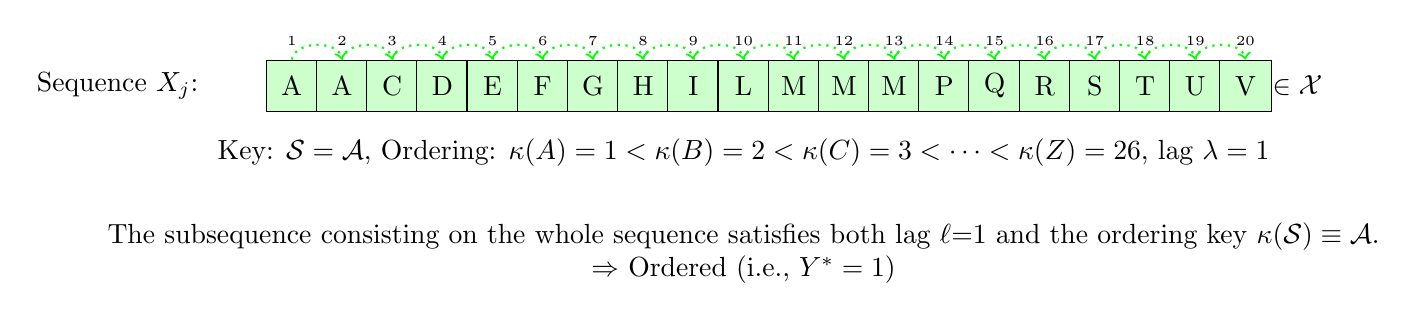
\begin{tikzpicture}[scale=0.85]
% Full sequence with key letters highlighted
\foreach \i/\letter in {1/A,2/A,3/C,4/D,5/E,6/F,7/G,8/H,9/I,10/L,11/M,12/M,13/M,14/P,15/Q,16/R,17/S,18/T,19/U,20/V} {           
    \node[draw,minimum size=0.65cm,text=black, fill=green!20] (n\i) at (\i*0.75,0) {\letter};
}
\node[anchor=east] at (-0.5,0) {Sequence $X_j$:};
\node[right=12cm of n1] {$\in \mathcal{X}$};

% Position numbers above key letters
\node[above=0.05cm of n1,black,font=\tiny] {1};
\node[above=0.05cm of n2,black,font=\tiny] {2};
\node[above=0.05cm of n3,black,font=\tiny] {3};
\node[above=0.05cm of n4,black,font=\tiny] {4};
\node[above=0.05cm of n5,black,font=\tiny] {5};
\node[above=0.05cm of n6,black,font=\tiny] {6};
\node[above=0.05cm of n7,black,font=\tiny] {7};
\node[above=0.05cm of n8,black,font=\tiny] {8};
\node[above=0.05cm of n9,black,font=\tiny] {9};
\node[above=0.05cm of n10,black,font=\tiny] {10};
\node[above=0.05cm of n11,black,font=\tiny] {11};
\node[above=0.05cm of n12,black,font=\tiny] {12};
\node[above=0.05cm of n13,black,font=\tiny] {13};
\node[above=0.05cm of n14,black,font=\tiny] {14};
\node[above=0.05cm of n15,black,font=\tiny] {15};
\node[above=0.05cm of n16,black,font=\tiny] {16};
\node[above=0.05cm of n17,black,font=\tiny] {17};
\node[above=0.05cm of n18,black,font=\tiny] {18};
\node[above=0.05cm of n19,black,font=\tiny] {19};
\node[above=0.05cm of n20,black,font=\tiny] {20};

% Key information - moved down more
\node at (7.5,-1) {Key: $\mathcal{S} = \mathcal{A}$, Ordering: $\kappa(A)=1 < \kappa(B)=2 < \kappa(C)=3 < \cdots < \kappa(Z)=26 $, lag $\lambda=1$};

% Arrows showing different paths - all starting lower and with better spacing

\draw[->,thick,green,dotted] (n1.north) to[out=80,in=100] (n2.north);
\draw[->,thick,green,dotted] (n2.north) to[out=80,in=100] (n3.north);
\draw[->,thick,green,dotted] (n3.north) to[out=80,in=100] (n4.north);
\draw[->,thick,green,dotted] (n4.north) to[out=80,in=100] (n5.north);
\draw[->,thick,green,dotted] (n5.north) to[out=80,in=100] (n6.north);
\draw[->,thick,green,dotted] (n6.north) to[out=80,in=100] (n7.north);
\draw[->,thick,green,dotted] (n7.north) to[out=80,in=100] (n8.north);
\draw[->,thick,green,dotted] (n8.north) to[out=80,in=100] (n9.north);
\draw[->,thick,green,dotted] (n9.north) to[out=80,in=100] (n10.north);
\draw[->,thick,green,dotted] (n10.north) to[out=80,in=100] (n11.north);
\draw[->,thick,green,dotted] (n11.north) to[out=80,in=100] (n12.north);
\draw[->,thick,green,dotted] (n12.north) to[out=80,in=100] (n13.north);
\draw[->,thick,green,dotted] (n13.north) to[out=80,in=100] (n14.north);
\draw[->,thick,green,dotted] (n14.north) to[out=80,in=100] (n15.north);
\draw[->,thick,green,dotted] (n15.north) to[out=80,in=100] (n16.north);
\draw[->,thick,green,dotted] (n16.north) to[out=80,in=100] (n17.north);
\draw[->,thick,green,dotted] (n17.north) to[out=80,in=100] (n18.north);
\draw[->,thick,green,dotted] (n18.north) to[out=80,in=100] (n19.north);
\draw[->,thick,green,dotted] (n19.north) to[out=80,in=100] (n20.north);

% Results - moved down even more
\node[align=center] at (7.5,-2.5) {The subsequence consisting on the whole sequence satisfies both lag $\ell$=1 and the ordering key $\kappa(\mathcal{S}) \equiv \mathcal{A}$.\\
$\Rightarrow$ Ordered (i.e., $Y^{*}=1$)};
\end{tikzpicture}
\caption{Sequence classification example using the \textit{naive} method. Key letters $\mathcal{S} = \mathcal{A}$ (i.e., all letters). Arrows show gaps between key letters. 
In green letters (and gaps) that do have lag-connections with other key letters and that satisfy the ordering $\kappa(\mathcal{S}) \equiv \mathcal{A}$. Note: in this example $n=20$, $m=26$.}
\label{fig:naive_example}
\end{figure}

\label{appendix:Figures}
\begin{figure}[h!]
\centering
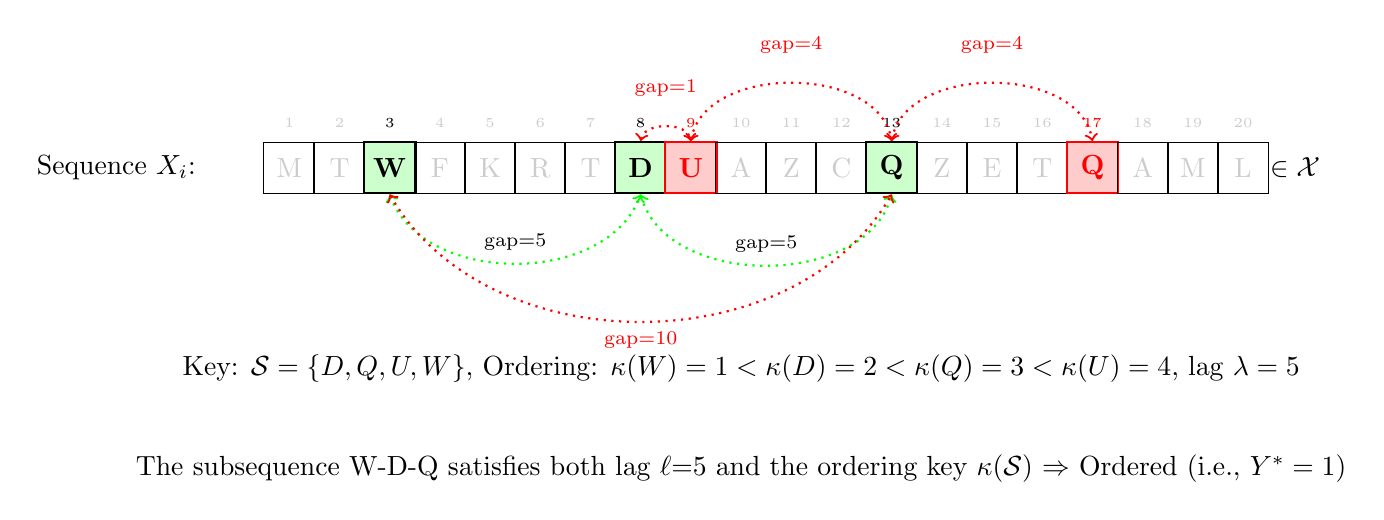
\begin{tikzpicture}[scale=0.85, baseline=(current bounding box.center)]
% Full sequence with key letters highlighted
\foreach \i/\letter in {1/M,2/T,3/W,4/F,5/K,6/R,7/T,8/D,9/U,10/A,11/Z,12/C,13/Q,14/Z,15/E, 16/T,17/Q,18/A,19/M,20/L} {
    % Check prima se è posizione 9 (rosso)
    \ifnum\i=9
        \node[draw,thick,red,minimum size=0.65cm,fill=red!20] (n\i) at (\i*0.75,0) {\textbf{\letter}};
    
    \else
        \ifnum\i=17
            \node[draw,thick,red,minimum size=0.65cm,fill=red!20] (n\i) at (\i*0.75,0) {\textbf{\letter}};
        \else
            % Altrimenti check se è 3, 8 o 13 (arancione)
            \pgfmathparse{\i==3 || \i==8 || \i==13 ? 1 : 0}
            \ifnum\pgfmathresult=1
                \node[draw,thick,black,minimum size=0.65cm,fill=green!20] (n\i) at (\i*0.75,0) {\textbf{\letter}};
            \else
                % Altrimenti grigio
                \node[draw,minimum size=0.65cm,text=gray!40] (n\i) at (\i*0.75,0) {\letter};
            \fi
        \fi
    \fi
}
\node[anchor=east] at (-0.5,0) {Sequence $X_i$:};
\node[right=12cm of n1] {$\in \mathcal{X}$};

% Position numbers above key letters
\node[above=0.05cm of n1,gray!40,font=\tiny] {1};
\node[above=0.05cm of n2,gray!40,font=\tiny] {2};
\node[above=0.05cm of n3,black,font=\tiny] {3};
\node[above=0.05cm of n4,gray!40,font=\tiny] {4};
\node[above=0.05cm of n5,gray!40,font=\tiny] {5};
\node[above=0.05cm of n6,gray!40,font=\tiny] {6};
\node[above=0.05cm of n7,gray!40,font=\tiny] {7};
\node[above=0.05cm of n8,black,font=\tiny] {8};
\node[above=0.05cm of n9,red,font=\tiny] {9};
\node[above=0.05cm of n10,gray!40,font=\tiny] {10};
\node[above=0.05cm of n11,gray!40,font=\tiny] {11};
\node[above=0.05cm of n12,gray!40,font=\tiny] {12};
\node[above=0.05cm of n13,black,font=\tiny] {13};
\node[above=0.05cm of n14,gray!40,font=\tiny] {14};
\node[above=0.05cm of n15,gray!40,font=\tiny] {15};
\node[above=0.05cm of n16,gray!40,font=\tiny] {16};
\node[above=0.05cm of n17,red,font=\tiny] {17};
\node[above=0.05cm of n18,gray!40,font=\tiny] {18};
\node[above=0.05cm of n19,gray!40,font=\tiny] {19};
\node[above=0.05cm of n20,gray!40,font=\tiny] {20};

% Key information - moved down more
\node at (7.5,-3) {Key: $\mathcal{S} = \{D, Q, U, W\}$, Ordering: $\kappa(W)=1 < \kappa(D)=2 < \kappa(Q)=3 < \kappa(U)=4$, lag $\lambda=5$};

% Arrows showing different paths - all starting lower and with better spacing
% Path 1: B to D (gap=5, red)
\draw[<->,thick,green,dotted] (n3.south) to[out=-70,in=-110] node[below,yshift=0.5cm,font=\scriptsize,black] {gap=5} (n8.south);

% Path 2: D to G (gap=4, green) 
\draw[<->,thick,green,dotted] (n8.south) to[out=-75,in=-105] node[below,yshift=0.5cm,font=\scriptsize,black] {gap=5} (n13.south);

% Path 3: B to G (gap=10, purple)
\draw[<->,thick,red,dotted] (n3.south) to[out=-60,in=-120] node[below,yshift=0cm,font=\scriptsize,red] {gap=10} (n13.south);

\draw[<->,thick,red,dotted] (n8.north) to[out=80,in=100] node[above,yshift=0.25cm,font=\scriptsize,red] {gap=1} (n9.north);

\draw[<->,thick,red,dotted] (n9.north) to[out=80,in=100] node[above,yshift=0.25cm,font=\scriptsize,red] {gap=4} (n13.north);

\draw[<->,thick,red,dotted] (n13.north) to[out=80,in=100] node[above,yshift=0.25cm,font=\scriptsize,red] {gap=4} (n17.north);

% Results - moved down even more
\node[align=center] at (7.5,-4.5) {The subsequence W-D-Q satisfies both lag $\ell$=5 and the ordering key $\kappa(\mathcal{S})$ 
$\Rightarrow$ Ordered (i.e., $Y^{*}=1$)};

\end{tikzpicture}
\caption{Sequence classification with \textit{tricky} method. Key letters $\mathcal{S} = (D, Q, U, W)$ are extracted from the full sequence (non-key in gray). Arrows indicate gaps. Red: letters/gaps without lag-connections to other keys. Green: letters/gaps with lag-connections satisfying ordering $\kappa(\mathcal{S})$. Here $n=20$, $m=4$.}

\label{fig:tricky_example}
\end{figure}

\begin{figure}[h!]
\centering
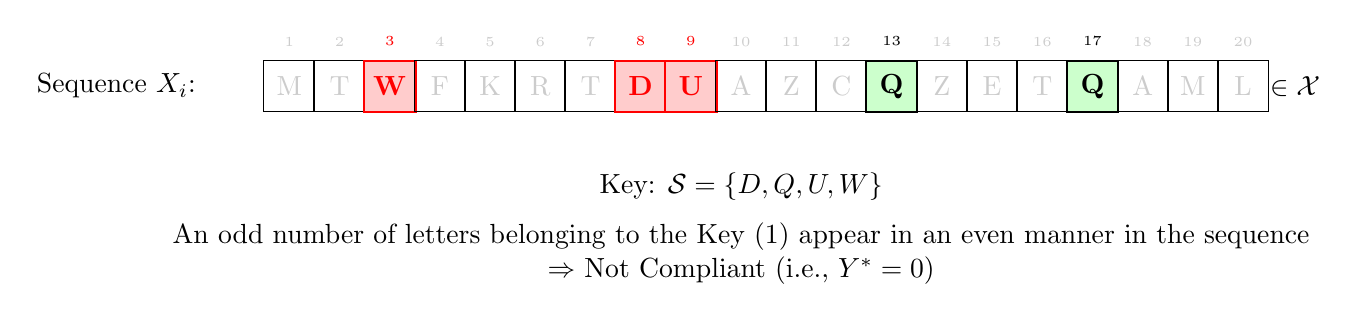
\begin{tikzpicture}[scale=0.85, baseline=(current bounding box.center)]
\foreach \i/\letter in {1/M,2/T,3/W,4/F,5/K,6/R,7/T,8/D,9/U,10/A,11/Z,12/C,13/Q,14/Z,15/E,16/T,17/Q,18/A,19/M,20/L} {
    \ifnum\i=3
        \node[draw,thick,red,minimum size=0.65cm,fill=red!20] (n\i) at (\i*0.75,0) {\textbf{\letter}};
    \else
        % D at position 8 (odd count -> red)
        \ifnum\i=8
            \node[draw,thick,red,minimum size=0.65cm,fill=red!20] (n\i) at (\i*0.75,0) {\textbf{\letter}};
        \else
            % U at position 9 (odd count -> red)
            \ifnum\i=9
                \node[draw,thick,red,minimum size=0.65cm,fill=red!20] (n\i) at (\i*0.75,0) {\textbf{\letter}};
            \else
                % Q at positions 13 and 17 (even count -> green)
                \pgfmathparse{\i==13 || \i==17 ? 1 : 0}
                \ifnum\pgfmathresult=1
                    \node[draw,thick,black,minimum size=0.65cm,fill=green!20] (n\i) at (\i*0.75,0) {\textbf{\letter}};
                \else
                    % Non-key letters in gray
                    \node[draw,minimum size=0.65cm,text=gray!40] (n\i) at (\i*0.75,0) {\letter};
                \fi
            \fi
        \fi
    \fi
}
\node[anchor=east] at (-0.5,0) {Sequence $X_i$:};
\node[right=12cm of n1] {$\in \mathcal{X}$};

% Position numbers above letters
\foreach \i in {1,...,20} {
    \pgfmathparse{\i==3 || \i==8 || \i==9 ? "red" : (\i==13 || \i==17 ? "black" : "gray!40")}
    \edef\nodecolor{\pgfmathresult}
    \node[above=0.05cm of n\i,\nodecolor,font=\tiny] {\i};
}

% Key information
\node at (7.5,-1.5) {Key: $\mathcal{S} = \{D, Q, U, W\}$};


% Result
\node[align=center] at (7.5,-2.5) {An odd number of letters belonging to the Key (1) appear in an even manner in the sequence \\
$\Rightarrow$ Not Compliant (i.e., $Y^{*}=0$)};

\end{tikzpicture}
\caption{Sequence classification example using the \textit{parity} method. Key letters $\mathcal{S} = \{D, Q, U, W\}$ are extracted from the full sequence (non-key letters in gray).
The parity criterion requires \emph{an even number of unique} key letter to appear an \textbf{even} number of times.
In green: key letters with even count. In red: key letters with odd count.
Since not all key letters have even counts, the sequence is labeled as non-compliant ($Y^{*}=1$).}
\label{fig:parity_example}
\end{figure}

\begin{figure}[htbp]
    \centering
    \begin{subfigure}[b]{0.48\textwidth}
        \centering
        
\includegraphics[width=\textwidth]{naive_ngrams.png}
        \caption{Naive}
        \label{fig:ngram_naive}
    \end{subfigure}
    \hfill
    \begin{subfigure}[b]{0.48\textwidth}
        \centering
        
\includegraphics[width=\textwidth]{parity_deterministic_ngram.png}
        \caption{Parity deterministic}
        \label{fig:ngram_parity}
    \end{subfigure}

    \vspace{0.5cm}

    \begin{subfigure}[b]{0.48\textwidth}
        \centering
        
\includegraphics[width=\textwidth]{csv_9_random-ngrams.png}
        \caption{Tricky random}
        \label{fig:ngram_tricky_random}
    \end{subfigure}
    \hfill
    \begin{subfigure}[b]{0.48\textwidth}
        \centering
        \includegraphics[width=\textwidth]{tricky_deterministic_ngrams.png}
        \caption{Tricky deterministic}
        \label{fig:ngram_tricky_det}
    \end{subfigure}
    \caption{Frequency distribution of the top-100 most discriminative $n$-grams ($n \in \{1,2,3,4,5,6\}$) by class label across the four synthetic datasets (\textit{blue} is ordered (i.e. Label=1), \textit{orange} unordered (i.e. Label=0)). In the \textit{naive} setting (a), discriminative signal concentrates in bigrams, with large frequency differences between classes and high absolute counts. Notably, disordered pairs produce \emph{illegal bigrams} that never appear in ordered sequences, providing an extremely strong signal for $n$-gram classifiers. The \textit{parity} methods (b) show a qualitatively different pattern. While some $k$-grams (particularly for $k=6$) appear exclusively for one class, visible as bars present for only one label, two factors limit their utility. First, these discriminative $k$-grams occur with very low absolute frequencies (often $\leq 10$ occurrences across $>400,000$ training examples). Second, there is a coverage problem: higher-order $k$-grams observed in training may simply not appear in test sequences. Lower-order $n$-grams (unigrams, bigrams) have inherently higher frequencies and coverage, being shorter, they are more likely to recur across both training and test sets. This creates a form of inherent ``data leakage'': not leakage due to methodological error, but a structural property of $n$-gram statistics where shorter patterns naturally generalize better, regardless of whether they capture the true underlying sequential mechanism. In contrast, \textit{tricky} methods (c, d) exhibit strong discriminative signal already at the unigram level: Label=0 sequences contain substantially more letter occurrences overall due to the outcome-dependent generation process, with the deterministic variant (e) showing the most pronounced class separation ($\sim$100k difference in 1-gram frequencies).}
    \label{fig:ngram_analysis}
\end{figure}


\begin{figure}
    \centering
    \includegraphics[width=1\linewidth]{naive_comparison.png}
        \caption{Model performance on the Naive dataset across four metrics. All models achieve near-perfect performance, with the exception of XGBoost. Shaded regions indicate variability across runs.}

    \label{fig:naive_comparison}
\end{figure}

\begin{figure}
    \centering
    \includegraphics[width=1\linewidth]{tricky_deterministic_comparison.png}
       \caption{Model performance on the Tricky Deterministic dataset across four metrics. Despite the deterministic label function ($\pi=0.0$), a clear separation emerges between model families. Bidirectional encoders (BERT, RoBERTa), recurrent architectures (LSTM, RNNTransformer), and larger causal decoders (Llama-8B) achieve near-perfect performance, demonstrating their ability to capture long-range dependencies when the relevant token can appear anywhere in the sequence. In contrast, smaller causal decoders (Llama-1B, Qwen-7B) plateau at $\sim$0.85 AUC, suggesting that autoregressive models require sufficient scale to compensate for the causal attention mask's limitation on integrating future context. Notably, the Llama-1M cold start model, trained from randomly-initialized weights, exhibits the same plateau, indicating that this capacity threshold is intrinsic to the architecture rather than an artifact of pretraining. The N-gram baseline saturates at $\sim$0.82, confirming that local patterns alone are insufficient. Shaded regions indicate variability across runs.}
    \label{fig:tricky_deterministic_comparison}
\end{figure}

\begin{figure}
    \centering
    \includegraphics[width=1\linewidth]{tricky_random_comparison.png}
        \caption{Model performance on the Tricky Random dataset across four metrics. The introduction of stochastic labels ($\pi=0.3$) establishes a optimal AUC of 0.67, providing an upper bound against which all models can be evaluated. Bidirectional encoders (BERT, RoBERTa), recurrent architectures (LSTM, Transformer, RNNTransformer), and larger causal decoders (Qwen-14B) approach this theoretical limit, confirming their capacity to extract the maximum learnable signal from the sequence. Smaller causal decoders (Llama-1B, Llama-8B, Qwen-4B) plateau at $\sim$0.58--0.60, near the N-gram baseline, suggesting that decoder-only models require substantially more parameters to overcome the autoregressive constraint under label noise. Interestingly, both XGBoost variants perform below chance ($<$0.50), indicating that their feature representations actively mislead the classifier, basic n-gram features fail to capture the relevant long-range dependency, while LLM embeddings appear to encode spurious correlations. This dataset highlights how label noise amplifies the parameter requirements for causal architectures to match bidirectional models. Shaded regions indicate variability across runs.}

    \label{fig:tricky_random}
\end{figure}


\begin{figure}
    \centering
    \includegraphics[width=1\linewidth]{parity_deterministic.png}
        \caption{Model performance on the Parity dataset across four metrics. Despite the deterministic label function ($\pi=0.0$), all models remain at chance level ($\sim$0.50 AUC), revealing a fundamental limitation shared across architectures. The parity task requires counting the occurrences of a target token modulo 2; a computation that demands precise tracking of state across the entire sequence. Neither bidirectional encoders (BERT, RoBERTa), recurrent architectures (LSTM, RNNTransformer), nor causal decoders (Llama, Qwen) show any learning signal, suggesting that current neural architectures struggle with tasks requiring exact counting or discrete state maintenance over long contexts. This result aligns with theoretical work on the expressiveness limitations of transformers for inherently sequential computations. The N-gram baseline also fails, as expected, since parity is a global property that cannot be inferred from local patterns. This task thus serves as a challenging benchmark that remains unsolved by standard fine-tuning approaches, pointing toward the need for architectural innovations or alternative training strategies to handle such computations. Shaded regions indicate variability across runs.}

    \label{fig:parity_task}
\end{figure}

\newpage

%%%%%%%%%%%%%%%%%%%%%%%
%% TABLES
%%%%%%%%%%%%%%%%%%%%%%%
\section{Tables}
\label{appendix:tables}

\begin{table}[h!]
\centering
\caption{N-gram baseline predictive performance across datasets. Results shown for optimized classification thresholds. \textit{Tricky Det.}: Deterministic sequence with statistical shortcuts. \textit{Tricky Rand.}: Same structure with added noise ($\pi=0.7$). \textit{Parity Det.}: Parity task requiring full sequence context.}
\label{tab:ngram_appendix}
\small
\begin{tabular}{lccccc|cccc|cccc}
\toprule
&&   \multicolumn{4}{c}{\textbf{Tricky Deterministic}} & \multicolumn{4}{c}{\textbf{Tricky Random}} & \multicolumn{4}{c}{\textbf{Parity Deterministic}} \\
\cmidrule(lr){3-6} \cmidrule(lr){7-10} \cmidrule(lr){11-14}
$n$ & Cov. Test  & AUC & F1 & Prec & Rec & AUC & F1 & Prec & Rec & AUC & F1 & Prec & Rec \\
\midrule
1 & 100.0\% & .813 & .645 & \textbf{.665} & \textbf{.626} & .585 & .593 & .422 & .996 & \textbf{.502} & \textbf{.668} & \textbf{.502} & \textbf{1.00} \\
2 & 100.0\% &\textbf{.819} & \textbf{.669} & .587 & .777 & \textbf{.586} & \textbf{.593} & .422 & \textbf{.998} & .498 & .668 & .502 & 1.00 \\
3 & 100.0\%  &.818 & .669 & .591 & .772 & .576 & .593 & \textbf{.423} & .993 & .497 & .668 & .502 & 1.00 \\
4 & 100.0\%  &.781 & .639 & .531 & .801 & .534 & .593 & .421 & 1.00 & .499 & .668 & .502 & 1.00 \\
5 & 41.67\% &.617 & .539 & .383 & .907 & .508 & .593 & .421 & 1.00 & .497 & .668 & .502 & 1.00 \\
6 & 1.9\% &.524 & .528 & .359 & .999 & .499 & .593 & .421 & 1.00 & .501 & .668 & .502 & 1.00 \\
7 & 0.1\% &.501 & .528 & .358 & 1.00 & .501 & .593 & .422 & 1.00 & .500 & .668 & .502 & 1.00 \\
\bottomrule
\end{tabular}
\end{table}

\begin{table}[h]
\centering
\caption{N-gram coverage between training and test sets. Analysis is common across all three synthetic datasets as they share identical sequences.}
\label{tab:ngram_coverage}
\small
\begin{tabular}{lrrr}
\toprule
$n$ & Unique Train & Unique Test & Coverage \\
\midrule
1 & 26 & 26 & 100.0\%\\
2 & 676 & 676 & 100.0\% \\
3 & 17,576 & 17,576 & 100.0\% \\
4 & 456,976 & 385,868 & 100.0\%  \\
5 & 4,948,910 & 773,862 & 41.7\% \\
6 & 5,942,184 & 749,024 & 1.9\%  \\
7 & 5,598,066 & 699,963 & 0.1\%  \\
\bottomrule
\end{tabular}
\vspace{0.1cm}

\footnotesize
\textit{Note:} Coverage represents the percentage of test n-grams that appear in the training set. Sharp drop at $n \geq 5$ indicates severe data sparsity, explaining baseline model collapse in Table~\ref{tab:ngram_appendix}.
\end{table}

\begin{table}[h]
\centering
\caption{N-gram analysis for the \textit{naive} dataset demonstrating information leakage through local patterns. At $n=20$, coverage drops to 0\%: no identical sequences exist between train and test sets, ruling out traditional data leakage. Yet discriminative signal persists at small $n$: bigrams achieve near-perfect AUC (0.999), confirming that ordering-based tasks leak information through local statistics (Theorem~\ref{thm:impossibility}). The AUC decrease for $n \geq 7$ reflects coverage sparsity rather than absence of signal.}
\label{tab:ngram_naive}
\small
\begin{tabular}{crrrr}
\toprule
$n$ & AUC & Unique Train & Unique Test & Coverage \\
\midrule
1 & 0.493 & 26 & 26 & 100.0\% \\
2 & 0.999 & 676 & 676 & 100.0\% \\
3 & 0.999 & 11,125 & 8,966 & 99.1\% \\
4 & 0.998 & 66,032 & 34,478 & 94.9\% \\
5 & 0.985 & 231,440 & 76,714 & 85.5\% \\
6 & 0.906 & 526,836 & 135,307 & 72.2\% \\
7 & 0.667 & 895,093 & 219,902 & 66.8\% \\
8 & 0.383 & 1,344,547 & 316,809 & 66.5\% \\
9 & 0.211 & 1,859,350 & 380,617 & 61.9\% \\
10 & 0.131 & 2,258,579 & 390,513 & 51.5\% \\
11 & 0.100 & 2,381,698 & 368,149 & 40.5\% \\
12 & 0.097 & 2,288,794 & 335,030 & 32.8\% \\
13 & 0.116 & 2,104,183 & 299,183 & 27.6\% \\
14 & 0.150 & 1,886,753 & 262,590 & 23.3\% \\
15 & 0.193 & 1,652,702 & 225,637 & 19.3\% \\
16 & 0.241 & 1,406,145 & 188,474 & 15.5\% \\
17 & 0.297 & 1,147,995 & 151,116 & 11.6\% \\
18 & 0.358 & 878,291 & 113,586 & 7.8\% \\
19 & 0.424 & 597,079 & 75,900 & 4.0\% \\
20 & 0.500 & 304,384 & 38,047 & 0.0\% \\
\bottomrule
\end{tabular}
\end{table}

\newpage

\section{Proofs}
\label{appendix:proof_theorems}

\begin{proof}[Proof of~\ref{paragraph:naive_setting}]
\label{proof:naive_setting}
In the naive setting, compliance requires $\mathcal{K}(X_1) \leq \mathcal{K}(X_2) \leq \cdots \leq \mathcal{K}(X_n)$. The number of such non-decreasing sequences equals the number of multisets of size $n$ from $\ell$ elements, which is $\binom{n+\ell-1}{n}$ by stars and bars formula. Dividing by the total $\ell^n$ sequences gives the result.
\end{proof}

\begin{proof}[Proof of Theorem~\ref{thm:optimal_performance}]
\label{proof:optimal_performance}
The label distribution conditional on compliance status $C \in \{0,1\}$ is $Y \mid C=1 \sim \mathrm{Bernoulli}(\pi)$ and $Y \mid C=0 \sim \mathrm{Bernoulli}(1-\pi)$. 

\emph{(a)} Given $C$, the optimal prediction is $\hat{Y} = C$ (predict 1 if compliant, 0 otherwise), achieving accuracy $P(\text{correct} \mid C=1) \cdot \rho + P(\text{correct} \mid C=0) \cdot (1-\rho) = \pi\rho + \pi(1-\rho) = \pi$.

\emph{(b)} The marginal $P(Y=1) = \rho\pi + (1-\rho)(1-\pi)$. For $\rho = 0.5$, this equals $0.5$, so both classes are equally likely and random guessing achieves $50\%$.

For AUC, we use the probabilistic interpretation of AUC.

\begin{equation}
AUC = P(s_+ > s_-) + \frac{1}{2} P(s_+ = s_-)
\end{equation}
where $s_+$ is the score for a random instance with $Y = 1$ and $s_-$ is the score for a random instance with $Y = 0$.

The Joint Distribution is:

\begin{align}
P(Y = 1, Y^* = 1) &= (1-\pi)\rho \\
P(Y = 1, Y^* = 0) &= \pi(1-\rho) \\
P(Y = 0, Y^* = 1) &= \pi\rho \\
P(Y = 0, Y^* = 0) &= (1-\pi)(1-\rho)
\end{align}

Marginal Distributions:

\begin{align}
P(Y = 1) &= \rho(1-\pi) + (1-\rho)\pi \\
P(Y = 0) &= \rho \pi + (1-\rho)(1-\pi)
\end{align}

Note that $P(Y = 1) + P(Y = 0) = 1$.

For the Conditional Score Distributions, define:
\begin{align}
    A &= P(s = 1 \mid Y = 1) = \frac{(1-\pi)\rho}{\rho(1-\pi) + (1-\rho)\pi} \\
    B &= P(s = 0 \mid Y = 1) = \frac{\pi(1-\rho)}{\rho(1-\pi) + (1-\rho)\pi} \\
    C &= P(s = 1 \mid Y = 0) = \frac{\pi\rho}{\rho \pi + (1-\rho)(1-\pi)} \\
    D &= P(s = 0 \mid Y = 0) = \frac{(1-\pi)(1-\rho)}{\rho \pi + (1-\rho)(1-\pi)}
\end{align}


    

Note: $A + B = 1$ and $C + D = 1$.

AUC Calculation:

\begin{align}
AUC &= A \cdot D + \frac{1}{2}(A \cdot C + B \cdot D) \\
&= A(1-C) + \frac{1}{2}A \cdot C + \frac{1}{2}(1-A)(1-C) \\
&= A - AC + \frac{1}{2}AC + \frac{1}{2} - \frac{1}{2}A - \frac{1}{2}C + \frac{1}{2}AC \\
&= \frac{1}{2} + \frac{1}{2}(A - C)
\end{align}

Simplification for Balanced Case:

For $\rho = 0.5$:
\begin{align}
A &= \frac{0.5(1-\pi)}{0.5(1-\pi) + 0.5\pi} = \frac{0.5(1-\pi)}{0.5} = 1-\pi \\
C &= \frac{0.5p}{0.5\pi + 0.5(1-\pi)} = \frac{0.5\pi}{0.5} = \pi
\end{align}

Therefore:
\begin{equation}
AUC = \frac{1}{2} + \frac{1}{2}[(1-\pi) - \pi] = \frac{1}{2} + \frac{1}{2}(1-2\pi) = 1 - \pi
\end{equation}

Alternatively, we can use the following expression.

Define $X = \rho(1-\pi) + (1-\rho)\pi$ and $Y = \rho \pi + (1-\rho)(1-\pi)$.

The numerator of $(A - C)$ can be computed as:
\begin{align}
(A - C) \cdot XY &= (1-\pi)\rho \cdot Y - \pi\rho \cdot X \\
&= \rho[(1-\pi)Y - \pi X] \\
&= \rho[(1-\pi)(\rho \pi + (1-\rho)(1-\pi)) - \pi(\rho(1-\pi) + (1-\rho)\pi)] \\
&= \rho[(1-\pi)^2(1-\rho) - \pi^2(1-\rho)] \\
&= \rho(1-\rho)[(1-\pi)^2 - \pi^2] \\
&= \rho(1-\rho)(1-2\pi)
\end{align}

Note: $(1-\pi)^2 - \pi^2 = 1 - 2\pi + \pi^2 - \pi^2 = 1 - 2\pi$.

Therefore:
\begin{equation}
A - C = \frac{\rho(1-\rho)(1-2\pi)}{XY}
\end{equation}

and
\begin{equation}
AUC = \frac{1}{2} + \frac{\rho(1-\rho)(1-2\pi)}{2XY}
\end{equation}
\qed

For F1, we use the Confusion Matrix with Respect to Observed Labels.

The classifier predicts $\hat{Y} = Y^*$ (the true label). Since we evaluate performance against the noisy observed labels $Y$, the confusion matrix elements are:

\begin{align}
\text{TP} &= P(\hat{Y} = 1 \cap Y = 1) = P(Y^* = 1 \cap Y = 1) \nonumber \\
&= P(Y = 1 \mid Y^* = 1) \cdot P(Y^* = 1) = (1-\pi)\rho \\
\text{FP} &= P(\hat{Y} = 1 \cap Y = 0) = P(Y^* = 1 \cap Y = 0) \nonumber \\
&= P(Y = 0 \mid Y^* = 1) \cdot P(Y^* = 1) = \pi\rho \\
\text{FN} &= P(\hat{Y} = 0 \cap Y = 1) = P(Y^* = 0 \cap Y = 1) \nonumber \\
&= P(Y = 1 \mid Y^* = 0) \cdot P(Y^* = 0) = \pi(1-\rho) \\
\text{TN} &= P(\hat{Y} = 0 \cap Y = 0) = P(Y^* = 0 \cap Y = 0) \nonumber \\
&= P(Y = 0 \mid Y^* = 0) \cdot P(Y^* = 0) = (1-\pi)(1-\rho)
\end{align}

For the Precision, by definition:
\begin{align}
\text{Precision} &= \frac{\text{TP}}{\text{TP} + \text{FP}} = \frac{(1-\pi)\rho}{(1-\pi)\rho + \pi\rho} \nonumber \\
&= \frac{(1-\pi)\rho}{\rho[(1-\pi) + \pi]} = \frac{(1-\pi)\rho}{\rho} = 1 - \pi
\end{align}

\textbf{Observation:} Precision is independent of the class distribution $\rho$ and depends only on the noise rate $\pi$.

For the Recall, by definition:
\begin{align}
\text{Recall} &= \frac{\text{TP}}{\text{TP} + \text{FN}} = \frac{(1-\pi)\rho}{(1-\pi)\rho + \pi(1-\rho)} \nonumber \\
&= \frac{(1-\pi)\rho}{\rho - \pi\rho + \pi - \pi\rho} = \frac{(1-\pi)\rho}{\rho(1-2\pi) + \pi}
\end{align}

\textbf{Verification for $\rho = 0.5$:}
\begin{equation}
\text{Recall} = \frac{(1-\pi) \cdot 0.5}{0.5(1-2\pi) + \pi} = \frac{0.5(1-\pi)}{0.5 - \pi + \pi} = \frac{0.5(1-\pi)}{0.5} = 1 - \pi
\end{equation}

Thus, for balanced classes, Precision $=$ Recall $= 1-\pi$.

For F1 Score, we use the definition, which is the harmonic mean of precision and recall:
\begin{equation}
F_1 = \frac{2 \cdot \text{Precision} \cdot \text{Recall}}{\text{Precision} + \text{Recall}}
\end{equation}

Substituting our expressions:
\begin{align}
F_1 &= \frac{2(1-\pi) \cdot \frac{(1-\pi)\rho}{\rho(1-2\pi) + \pi}}{(1-\pi) + \frac{(1-\pi)\rho}{\rho(1-2\pi) + \pi}} \nonumber \\
&= \frac{2(1-\pi)^2\rho}{(1-\pi)[\rho(1-2\pi) + \pi] + (1-\pi)\rho}
\end{align}

Simplifying the denominator:
\begin{align}
&(1-\pi)[\rho(1-2\pi) + \pi] + (1-\pi)\rho \nonumber \\
&= (1-\pi)\rho(1-2\pi) + \pi(1-\pi) + (1-\pi)\rho \nonumber \\
&= (1-\pi)\rho[(1-2\pi) + 1] + \pi(1-\pi) \nonumber \\
&= (1-\pi)\rho(2-2\pi) + \pi(1-\pi) \nonumber \\
&= (1-\pi)[2\rho(1-\pi) + \pi]
\end{align}

Therefore:
\begin{align}
F_1 &= \frac{2(1-\pi)^2\rho}{(1-\pi)[2\rho(1-\pi) + \pi]} = \frac{2(1-\pi)\rho}{2\rho(1-\pi) + \pi} \nonumber \\
&= \frac{2(1-\pi)\rho}{\pi + 2\rho(1-\pi)}
\end{align}

\textbf{Verification for $\rho = 0.5$:}
\begin{equation}
F_1 = \frac{2(1-\pi) \cdot 0.5}{\pi + 2 \cdot 0.5 \cdot (1-\pi)} = \frac{1-\pi}{\pi + (1-\pi)} = \frac{1-\pi}{1} = 1 - \pi
\end{equation}

\end{proof}

\subsection{Proof of Theorem~\ref{thm:impossibility}}
\label{appendix:proof_impossibility}

\begin{proof}
Let $\mathcal{C}_n \subset \mathcal{A}^n$ denote the set of sequentially compliant sequences of length $n$. Any compliant sequence is uniquely determined by the number of occurrences of each symbol, subject to the ordering constraint. By a standard stars-and-bars \citep{Stars_Bars} argument,
\[
|\mathcal{C}_n| = \binom{n + k - 1}{k - 1}.
\]

Fix the position $t=1$.  
Let $a_j \in \mathcal{A}$ be a symbol with rank $j = \kappa(a_j)$.  
If $X_1 = a_j$, then the remaining $n-1$ symbols must form a non-decreasing sequence over the alphabet $\{a_j, a_{j+1}, \dots, a_k\}$.  
The number of such sequences is
\[
|\mathcal{C}_{n,1,j}| = \binom{n - 1 + k - j}{k - j}.
\]

The conditional probability is therefore
\[
P(X_1 = a_j \mid Y = 1)
= \frac{|\mathcal{C}_{n,1,j}|}{|\mathcal{C}_n|}
= \frac{\binom{n - 1 + k - j}{k - j}}{\binom{n + k - 1}{k - 1}}.
\]
This quantity depends explicitly on $j$. In contrast, under the unconditional distribution,
\[
P(X_1 = a_j) = \frac{1}{k} \qquad \forall j.
\]
Hence there exists at least one $j$ such that
\[
P(X_1 = a_j \mid Y = 1) \neq P(X_1 = a_j).
\]

Since the conditional distribution of $X_1$ given $Y$ differs from its marginal distribution, it follows directly from the definition of mutual information that
\[
I(Y; X_1) > 0.
\]

\paragraph{Extension to infinite sequences.}
The result extends to infinite sequences by restriction to finite prefixes. For every $n$, the joint distribution of $(X_1,\dots,X_n)$ induced by the infinite process satisfies the hypotheses of Theorem~\ref{thm:impossibility}. Therefore, no limiting procedure can eliminate the local information induced by event-level ordering constraints.
\end{proof}



\subsection{Proof of Proposition \ref{prop:local-info-parity}}
\label{app:proof_prop_local_info}

To prove Proposition \ref{prop:local-info-parity}, we first introduce an auxiliary variable representing the standard parity of the sequence with respect to the subset $K$, and establish its local information properties.

\begin{lemma}[Auxiliary Parity Variable]
\label{lemma:standard_parity}
Define the variable $T := \left(\sum_{t=1}^n \mathbf{1}_{\{X_t \in K\}}\right) \mod 2$. 
Let $p = |K|/|\mathcal{A}|$. Then:
\begin{itemize}
    \item If $p = 1/2$, $I(T; X_t) = 0$ for all $t$.
    \item If $p \neq 1/2$, $I(T; X_t) \to 0$ as $n \to \infty$.
\end{itemize}
\end{lemma}

\begin{proof}[Proof of Lemma \ref{lemma:standard_parity}]
    Fix $t$ and write $S := \sum_{i=1}^n \mathbf{1}_{\{X_i \in K\}} = \mathbf{1}_{\{X_t \in K\}} + S_{-t}$, where $S_{-t} := \sum_{i \neq t} \mathbf{1}_{\{X_i \in K\}}$. 
    
    If $p=1/2$, $S_{-t} \pmod 2$ is uniform on $\{0,1\}$ (parity of $n-1$ fair coin flips). Thus, $P(T=1 | X_t = a) = 1/2 = P(T=1)$, implying $I(T; X_t) = 0$.
    
    If $p \neq 1/2$, let $q_n = P(S_{-t} \text{ is odd})$. We have $q_n = \frac{1 - (1-2p)^{n-1}}{2} \to \frac{1}{2}$ as $n \to \infty$. Consequently, the distribution of $T$ conditional on $X_t$ approaches uniformity, and $I(T; X_t) \to 0$.
\end{proof}

\medskip
\noindent \textbf{Completing the Proof of Proposition \ref{prop:local-info-parity}:}

Recall $Y = (\sum_{k \in K} \mathbf{1}_{\{N_k \text{ even}\}}) \mod 2$. Using the identity $\mathbf{1}_{\{n \text{ even}\}} = 1 \oplus (n \pmod 2)$ where $\oplus$ is addition modulo 2:
\begin{align*}
    Y &= \bigoplus_{k \in K} (1 \oplus (N_k \pmod 2)) \\
      &= \left(\bigoplus_{k \in K} 1\right) \oplus \left(\bigoplus_{k \in K} (N_k \pmod 2)\right).
\end{align*}
The first term is $|K| \pmod 2$. The second term is $(\sum_{k \in K} N_k) \pmod 2$, which is exactly $\sum_{t=1}^n \mathbf{1}_{\{X_t \in K\}} \pmod 2 = T$.
Thus:
\[
    Y = (|K| \pmod 2) \oplus T.
\]
For a fixed set $K$, the term $(|K| \pmod 2)$ is a constant. The mapping $T \mapsto Y$ is therefore a bijection (identity or bit-flip). Since mutual information is invariant under bijective transformations:
\[
    I(Y; X_t) = I(T; X_t).
\]
Applying Lemma \ref{lemma:standard_parity}, the statement follows. \qed
% ==================================================
% HYPERPARAMETER CONFIGURATION
% ==================================================
\section{Models and Hyperparameter Configurations}
\label{appendix:training}

This appendix provides complete hyperparameter configurations for all models evaluated in our experiments.

\subsection{Training Procedure}
\label{subsec:training}

\paragraph{Optimization.}
All neural models are trained using the AdamW optimizer~\citep{AdamW} with weight decay. For pretrained LLMs and BERT, we use a linear learning rate schedule with 6\% warmup steps. We employ cross-entropy loss for binary classification. Training uses early stopping based on validation loss with patience of 3 epochs for pretrained models and 5 epochs for models trained trained with randomly initialized parameters.

\paragraph{Pretrained models.}
LLMs (Llama, Qwen) and BERT are fine-tuned with learning rate $2 \times 10^{-5}$, batch size 16, and maximum sequence length 200 tokens. To enable efficient fine-tuning, we apply LoRA~\citep{LoRA} with rank $r=8$, $\alpha=16$, and dropout 0.1, targeting the attention projection matrices (\texttt{q\_proj}, \texttt{k\_proj}, \texttt{v\_proj}, \texttt{o\_proj} for LLMs; \texttt{query}, \texttt{key}, \texttt{value} for BERT). Large models employ gradient checkpointing and mixed-precision training (bfloat16) to fit within GPU memory constraints. We train for a maximum of 20 epochs with patience of 3 epochs.

\paragraph{Randomly initialized Models.}
LSTM, BiLSTM, Transformer, and hybrid architectures are trained with batch size 64 for up to 30 epochs. Learning rates are tuned per architecture: $10^{-3}$ for recurrent models (LSTM, BiLSTM), $5 \times 10^{-4}$ for Transformer-based models, and $10^{-4}$ for the BiLSTM-Transformer hybrid. Dropout rates range from 0.2 to 0.3 depending on model capacity. Early stopping monitors validation F1 score with patience of 5 epochs.

\paragraph{XGBoost baselines.}
XGBoost models use learning rate 0.05, maximum depth 6, subsample ratio 0.8, and column sampling ratio 0.8 per tree. We apply L1 regularization ($\alpha=0.5$) and L2 regularization ($\lambda=1.5$) with minimum child weight 2 and minimum split gain $\gamma=0.1$. Class imbalance is addressed via \texttt{scale\_pos\_weight}. Training runs for up to 200 boosting rounds with early stopping (patience 10) based on validation log-loss.

\paragraph{Threshold optimization.}
For all models, we optimize the classification threshold on the validation set by searching over $\{0.10, 0.11, \ldots, 0.89\}$ to maximize F1 score, rather than using the default 0.5 threshold.

\begin{table}[h]
\centering
\caption{Models tested and relative dimension. For XGBoost, we report hyperparameter configuration in Table~\ref{tab:xgboost_config}. As tree ensemble complexity is not directly comparable to neural network parameter counts, we omit this metric; the trained model typically comprised 80–120 trees with maximum depth 6.}
\label{tab:models}
\begin{tabular}{llr}
\toprule
Category & Model & Parameters \\
\midrule
\multirow{Pretrained} 
  & BERT-base & 110M \\
  & RoBERTa & 355M\\
  & Llama-3.2-1B & 1.0B \\
  & Qwen3-4B-Think & 4.0B\\
  & Llama-3.1-8B & 8.0B \\
  & Qwen2.5-14B & 14B \\
  & Llama-3.1-70B & 70B \\
  
\midrule
\multirow{Randomly initialized}
  & Llama-1M & 1M  \\
  & LSTM & 198K--340K \\
  & BiLSTM & 256K--395K \\
  & Transformer & 103K--104K \\
  & BiLSTM-Transformer & 319K--455K \\
\midrule
Tree-based & XGBoost & -- \\
\bottomrule
\end{tabular}
\end{table}


% ----------------------------------------------------------------------------
\subsection{Pretrained Language Models}
\label{appendix:pretrained}

Table~\ref{tab:llm_config} summarizes the fine-tuning configuration for pretrained LLMs.

\begin{table}[h]
\centering
\caption{Fine-tuning configuration for pretrained LLMs (Llama, Qwen).}
\label{tab:llm_config}
\begin{tabular}{ll}
\toprule
Hyperparameter & Value \\
\midrule
\multicolumn{2}{l}{\textit{Training}} \\
Learning rate & $2 \times 10^{-5}$ \\
Optimizer & AdamW \\
Batch size & 16 \\
Max epochs & 20 \\
Early stopping patience & 3 \\
Early stopping criterion & Validation loss \\
Warmup ratio & 6\% of total steps \\
Scheduler & Linear decay \\
\midrule
\multicolumn{2}{l}{\textit{LoRA Configuration}} \\
Rank ($r$) & 8 \\
Alpha ($\alpha$) & 16 \\
Dropout & 0.1 \\
Target modules & \texttt{q\_proj}, \texttt{k\_proj}, \texttt{v\_proj}, \texttt{o\_proj} \\
Bias & None \\
Task type & \texttt{CAUSAL\_LM} \\
\midrule
\multicolumn{2}{l}{\textit{Input Processing}} \\
Max sequence length & 512 tokens \\
Padding & Max length \\
Truncation & True \\
\midrule
\multicolumn{2}{l}{\textit{Memory Optimization}} \\
Precision & bfloat16 \\
Gradient checkpointing & Enabled \\
Use cache & Disabled \\
\bottomrule
\end{tabular}
\end{table}

Table~\ref{tab:tiny_llm_config} shows the architectural configurations for small-scale Llama models trained with randomly initialized parameters.

\begin{table}[h]
\centering
\caption{Architecture configurations for Llama models trained with randomly initialized parameters.}
\label{tab:tiny_llm_config}
\begin{tabular}{lrrrrr}
\toprule
Model & Hidden size & Layers & Heads & KV Heads & Intermediate size \\
\midrule
Llama-1M & 128 & 4 & 4 & 2 & 512 \\
\bottomrule
\end{tabular}
\end{table}

% ----------------------------------------------------------------------------
\subsection{BERT Models}
\label{appendix:bert}

Table~\ref{tab:bert_config} summarizes the fine-tuning configuration for BERT-based models.

\begin{table}[h]
\centering
\caption{Fine-tuning configuration for BERT models.}
\label{tab:bert_config}
\begin{tabular}{ll}
\toprule
Hyperparameter & Value \\
\midrule
\multicolumn{2}{l}{\textit{Training}} \\
Learning rate & $2 \times 10^{-5}$ \\
Optimizer & AdamW \\
Batch size & 16 \\
Max epochs & 20 \\
Early stopping patience & 3 \\
Early stopping criterion & Validation loss \\
Warmup ratio & 6\% of total steps \\
Scheduler & Linear decay \\
\midrule
\multicolumn{2}{l}{\textit{LoRA Configuration (when used)}} \\
Rank ($r$) & 8 \\
Alpha ($\alpha$) & 16 \\
Dropout & 0.1 \\
Target modules & \texttt{query}, \texttt{key}, \texttt{value} \\
Bias & None \\
Task type & \texttt{SEQ\_CLS} \\
\midrule
\multicolumn{2}{l}{\textit{Input Processing}} \\
Max sequence length & 512 tokens \\
Padding & Max length \\
Truncation & True \\
\bottomrule
\end{tabular}
\end{table}


% ----------------------------------------------------------------------------
\subsection{Recurrent and Transformer Architectures (Randomly Initialized)}
\label{appendix:dl_scratch}

Table~\ref{tab:dl_training} summarizes the training configuration shared across all models trained from scratch.

\begin{table}[h]
\centering
\caption{Training configuration for models trained with randomly initialized parameters.}
\label{tab:dl_training}
\begin{tabular}{ll}
\toprule
Hyperparameter & Value \\
\midrule
Optimizer & Adam \\
Batch size & 64 \\
Max epochs & 30 \\
Early stopping patience & 5 \\
Early stopping criterion & Validation F1 \\
Loss function & Cross-entropy \\
\bottomrule
\end{tabular}
\end{table}

Table~\ref{tab:dl_default_config} and Table~\ref{tab:dl_optimal_config} present the default and optimized architecture configurations, respectively.

\begin{table}[h]
\centering
\caption{Default architecture configurations for randomly initialized models.}
\label{tab:dl_default_config}
\begin{tabular}{llllll}
\toprule
Model & Embed. dim & Hidden dim & Layers & Dropout & Learning rate \\
\midrule
Transformer & 64 & 256 (FFN) & 2 & 0.3 & $5 \times 10^{-4}$ \\
LSTM & 32 & 64 & 2 & 0.3 & $10^{-3}$ \\
BiLSTM-Transformer & 64 & 64 (RNN) / 256 (FFN) & 1+2 & 0.3 & $5 \times 10^{-4}$ \\
\bottomrule
\end{tabular}
\end{table}

\begin{table}[h]
\centering
\caption{Optimized architecture configurations for models randomly initialized.}
\label{tab:dl_optimal_config}
\begin{tabular}{llllll}
\toprule
Model & Embed. dim & Hidden dim & Layers & Dropout & Learning rate \\
\midrule
Transformer & 64 & 128 (FFN) & 3 & 0.3 & $5 \times 10^{-4}$ \\
LSTM & 32 & 128 & 2 & 0.2 & $2 \times 10^{-3}$ \\
BiLSTM & 64 & 64 & 3 & 0.2 & $10^{-3}$ \\
BiLSTM-Transformer & 128 & 32 (RNN) / 256 (FFN) & 1+3 & 0.3 & $10^{-4}$ \\
\bottomrule
\end{tabular}
\end{table}

Additional architecture details:
\begin{itemize}
    \item \textbf{Transformer}: 4 attention heads; GELU activation; learnable positional encodings; mean pooling with padding mask.
    \item \textbf{LSTM}: Final hidden state used for classification.
    \item \textbf{BiLSTM-Transformer}: BiLSTM output projected to embedding dimension, then processed by Transformer encoder.
\end{itemize}

% ----------------------------------------------------------------------------
\subsection{XGBoost Baselines}
\label{appendix:xgboost}

Table~\ref{tab:xgboost_config} presents the XGBoost configuration.

\begin{table}[h]
\centering
\caption{XGBoost hyperparameter configuration.}
\label{tab:xgboost_config}
\begin{tabular}{ll}
\toprule
Hyperparameter & Value \\
\midrule
\multicolumn{2}{l}{\textit{Tree Parameters}} \\
Max depth & 6 \\
Min child weight & 1 \\
Gamma (min split loss) & 0.1 \\
Subsample & 0.8 \\
Column sample by tree & 0.8 \\
\midrule
\multicolumn{2}{l}{\textit{Regularization}} \\
L1 regularization ($\alpha$) & 0.5 \\
L2 regularization ($\lambda$) & 1.5 \\
\midrule
\multicolumn{2}{l}{\textit{Training}} \\
Learning rate ($\eta$) & 0.05 \\
Max boosting rounds & 200 \\
Early stopping patience & 10 \\
Early stopping criterion & Validation log-loss \\
Tree method & \texttt{hist} \\
\midrule
\multicolumn{2}{l}{\textit{Class Imbalance}} \\
Scale pos weight & $N_{\text{negative}} / N_{\text{positive}}$ \\
\bottomrule
\end{tabular}
\end{table}

For XGBoost-LLM, embeddings are extracted from Llama-3.2-1B using the prompt format described in Section~\ref{subsec:encoding}, with mean pooling over the last hidden layer (dimension 2048).

% ----------------------------------------------------------------------------
\subsection{Data Fractions}
\label{appendix:fractions}

To assess data efficiency, we train each model on the following fractions of the training set: $\{1\%, 10\%, 30\%, 50\%, 75\%, 100\%\}$. Subsampling is performed using stratified sampling to maintain class balance across all fractions.

\paragraph{Reproducibility.}
All experiments use a fixed random seed (9550) for data splitting, weight initialization, and stochastic optimization. Each configuration is run with three different seeds; we report means and standard deviations (see ~\ref{tab:results_summary}).

% ----------------------------------------------------------------------------
\subsection{Hardware and Software}
\label{appendix:hardware}

Experiments are conducted on a single NVIDIA A100 GPU (80GB). Fine-tuning Llama-8B requires approximately 128GB CPU memory with gradient checkpointing enabled. Training times range from minutes (small models, 1\% data) to several hours (Llama-8B, full data).

\begin{table}[h]
\centering
\caption{Full classification performance across models and datasets (100\% training data). Standard deviations in parentheses.}
\label{tab:results_full}
\small
\begin{tabular}{@{}lcccc@{}}
\toprule
Model & AUC & F1 & Prec & Rec \\
\midrule
\multicolumn{5}{@{}l}{\textit{Naive ($\pi=0.0$)}} \\
\textit{Optimal} & 1.000 & 1.000 & 1.000 & 1.000 \\
N-gram & .999 & .999 & .999 & .999 \\
XGBoost (basic) & .603 (.004) & .714 (.005) & .556 (.004) & .995 (.003) \\
XGBoost (LLM) & .502 (.004) & .536 (.008) & .501 (.004) & .577 (.010) \\
BERT & .999 (.001) & .999 (.001) & .999 (.001) & .999 (.001) \\
RoBERTa & .999 (.001) & .999 (.001) & .999 (.001) & .999 (.001) \\
Llama-3.2-1B & .999 (.001) & .999 (.001) & .999 (.001) & .999 (.001) \\
Llama-3.1-8B & .999 (.001) & .999 (.001) & .999 (.001) & .999 (.001) \\
Llama-1M (cold) & .999 (.001) & .999 (.001) & .999 (.001) & .999 (.001) \\
Qwen3-4B-Think & .999 (.001) & .999 (.001) & .999 (.001) & .999 (.001) \\
LSTM & .999 (.001) & .999 (.001) & .999 (.001) & .999 (.001) \\
Transformer & .999 (.001) & .999 (.001) & .999 (.001) & .999 (.001) \\
RNNTransformer & .999 (.001) & .999 (.001) & .999 (.001) & .999 (.001) \\
\midrule
\multicolumn{5}{@{}l}{\textit{Tricky Deterministic ($\pi=0.0$)}} \\
\textit{Optimal} & 1.000 & 1.000 & 1.000 & 1.000 \\
2-gram & .821 & .672 & .593 & .775 \\
XGBoost (basic) & .625 (.012) & .457 (.015) & .516 (.010) & .409 (.018) \\
XGBoost (LLM) & .494 (.010) & .399 (.012) & .353 (.008) & .459 (.015) \\
BERT & .999 (.001) & .999 (.001) & .999 (.001) & 1.000 (.001) \\
RoBERTa & .999 (.001) & .999 (.001) & .999 (.001) & 1.000 (.001) \\
Llama-3.2-1B & .846 (.015) & .695 (.018) & .623 (.020) & .785 (.022) \\
Llama-3.1-8B & .995 (.003) & .984 (.008) & .976 (.010) & .993 (.007) \\
Llama-1M (cold) & .832 (.012) & .686 (.015) & .605 (.018) & .791 (.020) \\
Qwen3-4B-Think & .850 (.014) & .701 (.016) & .620 (.017) & .800 (.020) \\
LSTM & .999 (.001) & .994 (.003) & .995 (.003) & .994 (.003) \\
Transformer & .999 (.001) & .992 (.002) & .985 (.005) & 1.000 (.001) \\
RNNTransformer & .997 (.002) & .992 (.003) & .985 (.005) & 1.000 (.002) \\
\midrule
\multicolumn{5}{@{}l}{\textit{Tricky Random ($\pi=0.3$)}} \\
\textit{Optimal} & .670 & .577 & .700 & .491 \\
2-gram & .585 & .592 & .420 & 1.000 \\
XGBoost (basic) & .463 (.010) & .418 (.012) & .437 (.008) & .400 (.015) \\
XGBoost (LLM) & .418 (.011) & .453 (.014) & .437 (.008) & .470 (.018) \\
BERT & .669 (.006) & .592 (.004) & .420 (.005) & 1.000 (.002) \\
RoBERTa & .652 (.008) & .592 (.003) & .420 (.005) & 1.000 (.002) \\
Llama-3.2-1B & .587 (.008) & .592 (.005) & .420 (.006) & .999 (.005) \\
Llama-3.1-8B & .575 (.008) & .591 (.005) & .425 (.006) & .968 (.010) \\
Qwen3-4B-Think & .597 (.007) & .591 (.004) & .423 (.005) & .979 (.008) \\
Qwen2.5-14B$^{*}$ & .670 (---) & .586 (---) & .476 (---) & .763 (---) \\
LSTM & .665 (.003) & .562 (.020) & .660 (.002) & .489 (.031) \\
Transformer & .671 (.001) & .579 (.003) & .701 (.015) & .492 (.012) \\
RNNTransformer & .671 (.005) & .578 (.005) & .683 (.010) & .501 (.005) \\
\midrule
\multicolumn{5}{@{}l}{\textit{Parity Deterministic ($\pi=0.0$)}} \\
\textit{Optimal} & 1.000 & 1.000 & 1.000 & 1.000 \\
1-gram & .505 & .668 & .501 & 1.000 \\
XGBoost (basic) & .495 (.004) & .490 (.005) & .497 (.003) & .484 (.006) \\
XGBoost (LLM) & .501 (.003) & .639 (.005) & .502 (.002) & .881 (.008) \\
BERT & .503 (.002) & .668 (.002) & .501 (.002) & 1.000 (.001) \\
RoBERTa & .501 (.003) & .668 (.002) & .501 (.002) & 1.000 (.001) \\
Llama-3.2-1B & .497 (.005) & .668 (.001) & .501 (.002) & 1.000 (.001) \\
Llama-3.1-8B & .500 (.003) & .668 (.006) & .501 (.002) & 1.000 (.001) \\
Llama-1M (cold) & .503 (.003) & .668 (.002) & .501 (.003) & 1.000 (.001) \\
Llama-3.3-70B$^{*}$ & .502 (---) & .668 (---) & .501 (---) & 1.000 (---) \\
Qwen3-4B-Think & .500 (.002) & .668 (.003) & .501 (.000) & 1.000 (.001) \\
LSTM & .502 (.003) & .668 (.002) & .501 (.002) & 1.000 (.001) \\
Transformer & .501 (.003) & .668 (.002) & .501 (.002) & 1.000 (.001) \\
RNNTransformer & .501 (.002) & .668 (.001) & .501 (.003) & 1.000 (.001) \\
\bottomrule
$^{*} \text{just one run for time constraint, no standard deviation.}$
\end{tabular}
\end{table}


% \section{Effect of Label Noise}
% \label{appendix:noise}

% We analyze how label noise $\pi$ affects $k$-gram classifier performance and discuss potential pitfalls in experimental design.

% \subsection{Noise Model}

% Let $Y^*$ denote the true (noiseless) label and $Y$ the observed label. With noise rate $\pi \in [0, 0.5]$:
% \[
% Y = \begin{cases}
% Y^* & \text{with probability } 1 - \pi \\
% 1 - Y^* & \text{with probability } \pi
% \end{cases}
% \]

% This symmetric noise model flips labels independently with probability $\pi$.

% \subsection{Effect on Observed Class Balance}

% Let $\rho_{\text{int}} = P(Y^* = 1)$ denote the intrinsic compliance probability (determined by task parameters $m, \lambda, n, \ell$). The observed compliance probability is:
% \begin{equation}
% \rho_{\text{obs}} = \rho_{\text{int}} (1 - \pi) + (1 - \rho_{\text{int}}) \pi = \rho_{\text{int}} + \pi (1 - 2\rho_{\text{int}})
% \label{eq:rho-noisy}
% \end{equation}

% \subsection{Effect on Discriminability}

% Label noise attenuates the discriminability index:
% \begin{equation}
% d'_{\text{noisy}} = d'_{\text{clean}} \cdot (1 - 2\pi)
% \label{eq:dprime-noisy}
% \end{equation}

% \begin{proof}
% Under noise, the score distributions become mixtures. For the positive class:
% \[
% S^+_{\text{noisy}} = (1-\pi) S^+ + \pi S^-
% \]
% The mean shifts: $\mu^+_{\text{noisy}} = (1-\pi)\mu^+ + \pi\mu^-$. Similarly for the negative class. The difference:
% \[
% \mu^+_{\text{noisy}} - \mu^-_{\text{noisy}} = (1 - 2\pi)(\mu^+ - \mu^-)
% \]
% yielding $d'_{\text{noisy}} = (1 - 2\pi) d'_{\text{clean}}$.
% \end{proof}

% At $\pi = 0.5$ (maximum noise), $d' = 0$ regardless of the underlying task structure.

% \subsection{Degenerate Case: $\rho_{\text{int}} \approx 0$ with $\pi = 0.5$}
% \label{subsec:degenerate}

% A particularly problematic configuration arises when:
% Here, $\rho_{\text{int}} \approx 0$, indicating that only a negligible fraction of sequences are intrinsically compliant, while $\pi = 0.5$ implies that half of the labels are flipped.

% From Eq.~\eqref{eq:rho-noisy}: $\rho_{\text{obs}} = 0 + 0.5 \cdot 1 = 0.5$.

% This configuration is \textbf{misleading}: despite an apparently balanced dataset ($\rho_{\text{obs}} = 0.5$), no learnable structure is present, since all positive labels are noise-induced. As a result, both $k$-gram baselines and trained models attain $\text{AUC} \approx 0.5$, rendering this regime indistinguishable from a genuinely hard task.

% \paragraph{Diagnostic.}
% To distinguish ``hard task'' from ``destroyed signal'', as a diagnostic, one computes $\rho_{\text{int}}$ from the task parameters (Section~\ref{subsec:task-formulation}); when $\rho_{\text{int}} \ll \rho_{\text{obs}}$, the positive class is noise-dominated. Setting $\pi = 0$ provides a sanity check: an AUC close to $0.5$ indicates intrinsic task difficulty.

% \subsection{Recommended Practice}

% For controlled sequential reasoning experiments, primary evaluations should be conducted at $\pi = 0$ to ensure a clean signal. When label noise is present ($\pi > 0$), $\rho_{\text{int}}$ should be reported in addition to $\rho_{\text{obs}}$, and verified to lie within a non-degenerate range (e.g., $0.1 < \rho_{\text{int}} < 0.9$). Noise robustness can then be assessed by varying $\pi$ independently while holding $\rho_{\text{int}}$ fixed.

% Table~\ref{tab:noise-effect} illustrates the effect of $\pi$ on a fixed task configuration.

% \begin{table}[h]
% \centering
% \caption{Effect of noise $\pi$ on bigram classifier AUC ($m=6$, $\lambda=3$, $\rho_{\text{int}} = 0.49$).}
% \label{tab:noise-effect}
% \footnotesize
% \begin{tabular}{c|ccc}
% \toprule
% $\pi$ & $\rho_{\text{obs}}$ & $d'_{\text{noisy}}/d'_{\text{clean}}$ & AUC (predicted) \\
% \midrule
% 0.00 & 0.49 & 1.00 & 0.72 \\
% 0.10 & 0.49 & 0.80 & 0.66 \\
% 0.20 & 0.49 & 0.60 & 0.60 \\
% 0.30 & 0.49 & 0.40 & 0.56 \\
% 0.40 & 0.49 & 0.20 & 0.53 \\
% 0.50 & 0.49 & 0.00 & 0.50 \\
% \bottomrule
% \end{tabular}
% \end{table}



%%%%%%%%%%%%%%%%%%%%%%%%%%%%%%%%%%%%%%%%%%%%%%%%%%%%%%%%%%%%%%%%%%%%%%%%%%%%%%%
%%%%%%%%%%%%%%%%%%%%%%%%%%%%%%%%%%%%%%%%%%%%%%%%%%%%%%%%%%%%%%%%%%%%%%%%%%%%%%%


\end{document}


% This document was modified from the file originally made available by
% Pat Langley and Andrea Danyluk for ICML-2K. This version was created
% by Iain Murray in 2018, and modified by Alexandre Bouchard in
% 2019 and 2021 and by Csaba Szepesvari, Gang Niu and Sivan Sabato in 2022.
% Modified again in 2023 and 2024 by Sivan Sabato and Jonathan Scarlett.
% Previous contributors include Dan Roy, Lise Getoor and Tobias
% Scheffer, which was slightly modified from the 2010 version by
% Thorsten Joachims & Johannes Fuernkranz, slightly modified from the
% 2009 version by Kiri Wagstaff and Sam Roweis's 2008 version, which is
% slightly modified from Prasad Tadepalli's 2007 version which is a
% lightly changed version of the previous year's version by Andrew
% Moore, which was in turn edited from those of Kristian Kersting and
% Codrina Lauth. Alex Smola contributed to the algorithmic style files.
